% !TeX root = ../../Book1.tex
% 纲要标题：## 附录 E　反射群与多面体几何
% 纲要位置：几何学计划纲要.md，第 1002 行。
% 正文状态：五节及全部二十四小节初稿完成，含证明、模型计算与完整习题解答；尚未正式审核。
% 证明范围与外部输入：本附录从有限维凸几何和第19章的根、Weyl 群出发，建立反射群与多面体的代表模型；完整处理秩二及经典族计算、所选 Cauchy 刚性证明和 Dehn 不变量算例。一般有限型分类及剪刀合同的充分性理论准确外引，不重复第19章已有基础。

% 纲要内容开始
% 
% > 本附录证明范围与外部输入：本附录从有限维凸几何和第19章的根、Weyl 群出发，建立反射群与多面体的代表模型；完整处理秩二及经典族计算、所选 Cauchy 刚性证明和 Dehn 不变量算例。一般有限型分类及剪刀合同的充分性理论准确外引，不重复第19章已有基础。
% 
% * **有限反射群与根系**
%   * 正交反射、反射超平面与基本室
%   * 有限反射群的根系模型
%   * 晶体型与非晶体型的区别
%   * 紧 Lie 群的根系与 Weyl 群
% 
% * **单根、Dynkin 图与 Coxeter 图**
%   * 单根、正根与简单反射
%   * Cartan 整数与 Dynkin 图
%   * Coxeter 关系与反射角
%   * 秩二反射群与经典根系
%   * 有限反射群的分类
% 
% * **反射对称与正多胞形**
%   * 面格、旗与正多胞形
%   * 单纯形、立方体与交叉多胞形
%   * 三维正多面体的构造
%   * 反射群作用、基本室与对偶
%   * 正二十四胞体
% 
% * **凸多面体的整体刚性**
%   * 面度量、组合对应与刚性问题
%   * 凸多面体的球面链接
%   * Cauchy 变号引理
%   * Cauchy 凸多面体刚性定理
%   * 凸性条件与光滑曲面刚性的比较
% 
% * **Dehn 不变量与剪刀合同**
%   * 多面体剖分与剪刀合同
%   * 棱长、二面角与 Dehn 不变量
%   * 切割可加性与剖分不变性
%   * 立方体与正四面体的剪拼障碍
%   * 三维剪刀合同的分类
% 
% ---
% 
% 纲要内容结束

\chapter{反射群与多面体几何}
\label{g1:app:E}
\BookChapterNumber{g1:app:E}

\begin{chapterabstract}
	多面体的对称、刚性与剪拼问题，都把有限的局部数据同整体形状联系起来。本附录先用反射超平面及其法向根描述有限对称，证明单根与基本室的性质，计算秩二系统和四个经典族，再以旗的传递性构造正多胞形。随后从顶点的球面链接证明 Cauchy 凸多面体刚性定理，说明面形状与组合对应怎样确定三维凸实现。最后构造 Dehn 不变量，证明其剖分可加性，并用正四面体与同体积立方体说明三维剪拼中体积条件的不足。一般分类与剪刀合同充分性所需的外部结论在相应位置注明。
\end{chapterabstract}

\begin{learninggoals}
	\begin{itemize}
		\item 从正交反射构造根系，区分有限实根系与晶体根系，解释根长与反射超平面的不同作用。
		\item 证明单根、正根和基本室的性质，在秩二及经典族中计算 Cartan 矩阵、Coxeter 关系、群阶与根数。
		\item 用面格与旗定义正多胞形，核验三维五种正多面体及四维正二十四胞体的构造和对偶。
		\item 把顶点处的面角、二面角转写为球面链接的边长与内角，完成凸多面体整体刚性的证明。
		\item 定义 Dehn 不变量的取值空间，证明切割可加性，计算同体积而不剪刀合同的实例。
	\end{itemize}
\end{learninggoals}

立方体的六个面都相同，沿对称平面反射后，整个立方体仍与自身重合。若改问如何从六个正方形面组成立方体，仅知道每块面的形状还不够直接读出它们在空间中的位置；相邻面之间的角度也需要确定。再把这个立方体切开，允许各片移动和重新拼合，问题又变成：哪些别的多面体可以由同一批材料拼成？这三个问题分别关心保留整个对象的对称、保留各面形状的刚性，以及保留有限剖分的剪刀合同。

\ProseParagraphBreak

反射提供了理解有限对称的一种具体方法。一面镜子由超平面给出，反射公式只需要一个法向量；有限个镜面把空间分成若干室，选定一室后，可以用其墙的法向根恢复整个反射群。由此得到的矩阵和图，又能帮助组织正多胞形的面与对称。刚性与剪拼则使用不同的数据：前者在每个顶点附近比较二面角的增减，后者把沿棱的长度与角度配对。相同的多面体因问题不同，需要保留的信息也不同。

\ProseParagraphBreak

本附录主要使用\chapref{g1:ch:01}的 Euclid 等距变换、\chapref{g1:ch:03}的有限维凸性与多胞形，以及内积和有限群作用的基本计算。根与 Weyl 群的联系接续\chapref{g1:ch:19}，但有限反射群的构造从定义开始；刚性部分会恢复所需球面几何，Dehn 不变量所用的有理张量积也在使用前说明。因此，读者可以先读反射与正多胞形，也可以在回顾凸几何后直接读刚性及剪刀合同两节。

\ProseParagraphBreak

证明范围包括单根和基本室的基础结论、秩二与经典族的计算、所列正多胞形模型、Cauchy 刚性以及 Dehn 不变量的必要性与算例。一般 Coxeter 展示和有限反射群分类引用 Davis 的结果；体积与 Dehn 不变量相等蕴含有限剪刀合同的充分性引用 Sydler 的定理。

\section{有限反射群与根系}
\label{g1:sec:E01}

镜面对称可以把一个小区域的形状重复到整个图形上。一个正三角形有三条对称轴，沿轴反射的复合又产生旋转；以共同中心为原点，它们都由 Euclid 空间中的正交线性变换描述。本节从镜面和法向量出发，说明如何用有限个向量记录全部反射，并把这一模型与第19章的根联系起来。

\subsection{正交反射、反射超平面与基本室}
\label{g1:subsec:E01:01}

设 \(E\) 是有限维实内积空间，\(\alpha\in E\setminus\{0\}\)。每个向量都唯一分成沿 \(\alpha\) 的分量与垂直于 \(\alpha\) 的分量。保留后者、把前者变号，就得到
\begin{equation}\label{g1:eq:finite-root-reflection}
	s_\alpha(x)=x-\frac{2\langle x,\alpha\rangle}{\langle\alpha,\alpha\rangle}\alpha.
\end{equation}
它固定超平面 \(H_\alpha=\alpha^\perp\) 中的每个点，将 \(\alpha\) 送到 \(-\alpha\)，并保持内积。因此 \(s_\alpha^2=I\)、\(\det s_\alpha=-1\)；对任意非零实数 \(c\)，还有 \(s_{c\alpha}=s_\alpha\)。反射由超平面决定，法向量的长度尚不是这项变换的数据。

\begin{definition}[有限实反射群]\label{g1:def:finite-real-reflection-group}
	设 \(E\) 是有限维实内积空间。由若干形如\eqref{g1:eq:finite-root-reflection}的正交反射生成的有限子群 \(W\subset O(E)\)，称为\term[youxianshifanshequn]{有限实反射群}[finite real reflection group]。群内所有反射的固定超平面组成有限集合 \(\mathcal H\)，称为其\term[fanshechaopingmianpailie]{反射超平面排列}[reflection hyperplane arrangement]。开集
	\[
		E\setminus\bigcup_{H\in\mathcal H}H
	\]
	的连通分支称为\term[fansheshi]{室}[chamber]；选定其中一个作为\term[jibenshi]{基本室}[fundamental chamber]。室闭包的余维一面称为墙。
\end{definition}

这里的反射超平面都经过原点；附录 B 中含平移的晶体群则作用在整个仿射空间，两类问题的基本区域不能混用。若 \(W\) 有共同固定子空间 \(F=E^W\)，所有反射法向量都在 \(F^\perp\)，并张成 \(F^\perp\)：一个向量垂直于全部法向量，当且仅当它被所有生成反射固定。于是可以分开恒等作用的因子 \(F\)，只在 \(F^\perp\) 中研究反射。以下根系所处空间就是这个实际被根张成的空间。

\begin{proposition}[室的半空间表示与相邻反射]\label{g1:prop:finite-reflection-chambers}
	设 \(W\subset O(E)\) 为有限实反射群。对一个室 \(C\)，取 \(a\in C\)，并为每个 \(H\in\mathcal H\) 选择满足 \(\langle a,\alpha_H\rangle>0\) 的法向量。则
	\[
		C=\{x:\langle x,\alpha_H\rangle>0\ (H\in\mathcal H)\},\qquad
		\overline C=\{x:\langle x,\alpha_H\rangle\ge0\ (H\in\mathcal H)\}.
	\]
	室是开凸多面锥。隔着一面墙相邻的两个室由该墙的反射交换，且 \(W\) 在所有室上作用传递。
\end{proposition}
\begin{proof}
	在一个连通分支内，每个连续函数 \(x\mapsto\langle x,\alpha_H\rangle\) 的符号不变。上述严格不等式的公共解集又凸、非空，因而连通，故恰为 \(C\)。非严格不等式的解 \(x\) 可以由 \(x+ta\)、\(t>0\) 逼近，而这些点都在 \(C\)，这证明闭包公式。

	正交变换满足 \(ws_\alpha w^{-1}=s_{w\alpha}\)，所以 \(W\) 置换整个排列。若两室隔墙 \(H\) 相邻，在墙的相对内部选取不属于其他超平面的点，充分小的邻域只被 \(H\) 分成两半。反射固定墙、交换两半，又置换室，因此交换这两个相邻室。

	最后，对任意两室，选取连接其内点的线段，使线段不经过两个不同排列超平面的交。这可以做到：固定起点后，导致线段经过某个余维至少二的交空间的终点，落在一个真仿射子空间内；有限个这样的子空间不能覆盖目标室。线段逐次穿过有限面墙，把相应反射依次复合，就将第一室送到第二室。
\end{proof}

因此 \(W\overline C=E\)，每条轨道至少与 \(\overline C\) 相交。要把闭室作为基本区域，还需证明每条轨道在其中恰有一个代表。\cref{g1:thm:reflection-chamber-fundamental}将由镜面分隔证明这一点，并证明群元素对开室的作用是自由的。

\begin{example}[坐标反射与正交象限]\label{g1:eg:coordinate-reflection-chambers}
	在 \(\mathbb R^r\) 中，\(s_{e_i}\) 只改变第 \(i\) 个坐标的符号。这些反射相互交换，生成 \(2^r\) 个对角矩阵 \(\operatorname{diag}(\varepsilon_1,\ldots,\varepsilon_r)\)，其中 \(\varepsilon_i=\pm1\)。它们的室就是 \(2^r\) 个开象限，闭正象限与每条轨道恰交于 \((|x_1|,\ldots,|x_r|)\)。边界上的点可以被若干反射固定，因而闭室的像允许共享边界。
\end{example}

\subsection{有限反射群的根系模型}
\label{g1:subsec:E01:02}

镜面是一组超平面；要计算反射矩阵和夹角，选取法向量通常更方便。为了在反射后继续用同一组数据计算，反射一个法向量应当仍得到其中的向量。下面把这一要求写成有限向量集的条件。

\begin{definition}[有限约化实根系]\label{g1:def:finite-real-root-system}
	设 \(E\) 为正维有限维实内积空间。有限集合 \(\Phi\subset E\setminus\{0\}\) 若张成 \(E\)，并满足
	\[
		\Phi\cap\mathbb R\alpha=\{\alpha,-\alpha\},\qquad
		s_\alpha\Phi=\Phi\qquad(\alpha\in\Phi),
	\]
	就称为本附录所用的\term[youxianyuehuashigenxi]{有限约化实根系}[finite reduced real root system]。其中的向量称为根；第一项条件称为约化性。记
	\[
		W(\Phi)=\langle s_\alpha:\alpha\in\Phi\rangle.
	\]
	此定义暂不要求任何整数条件。
\end{definition}

\begin{proposition}[由群取根与由根取群]\label{g1:prop:reflection-root-model}
	有限约化实根系 \(\Phi\subset E\) 生成有限实反射群 \(W(\Phi)\)。反过来，若有限实反射群 \(W\subset O(E)\) 的共同固定空间为零且 \(E\ne0\)，则在每个反射超平面的两侧各取一个单位法向量，所得集合 \(\Phi_W\) 是有限约化实根系，并满足 \(W(\Phi_W)=W\)。
\end{proposition}
\begin{proof}
	每个生成反射都置换有限集 \(\Phi\)，所以得到同态 \(W(\Phi)\to\operatorname{Sym}(\Phi)\)。若元素固定全部根，就因根张成 \(E\) 而等于恒等变换。因此同态单射，群有限。

	反方向中，不同超平面的法线不同，故单位法向量满足约化性。若向量垂直于全部这些法向量，它被全部生成反射固定，按假设只能为零，所以法向量张成 \(E\)。对 \(w\in W\)，共轭公式把反射超平面 \(H\) 送到 \(wH\)，而 \(w\) 保持单位长度，故置换 \(\Phi_W\)。特别地，每个根反射保持 \(\Phi_W\)。由这些根得到的反射恰是 \(W\) 中的全部反射，因而生成原群。
\end{proof}

这一单位法向量模型保留了镜面和群，但未必保留 Lie 理论中的根长度。例如 \(B_r\) 的短根长度为 \(1\)，长根长度为 \(\sqrt2\)；把它们全部单位化不会改变任何反射，却会改变下一小节的整数条件。讨论反射群时可以归一化镜面的法向量，讨论给定根系时则须同时保留相对长度。

\begin{example}[正三角形的六根模型]\label{g1:eg:a2-reflection-model}
	在 \(E=\{x\in\mathbb R^3:x_1+x_2+x_3=0\}\) 中取
	\[
		\Phi=\{e_i-e_j:1\le i\ne j\le3\}.
	\]
	它由六个长度均为 \(\sqrt2\) 的向量组成。代入反射公式可见，\(s_{e_i-e_j}\) 交换坐标 \(x_i,x_j\)，保留其余坐标，因而置换根集。三个坐标交换生成 \(S_3\)，其在 \(E\) 上的作用忠实：若置换固定全部差向量，就固定全部坐标指标。因此 \(W(\Phi)\cong S_3\)，阶为六。三面反射墙是 \(x_i=x_j\)，六个室由三个坐标的六种严格排列确定；例如 \(x_1>x_2>x_3\) 给出一个开角为 \(\pi/3\) 的室。
\end{example}

\subsection{晶体型与非晶体型的区别}
\label{g1:subsec:E01:03}

有限性只要求反射重复后回到有限个方向；晶体条件还要求根之间的系数可以用整数记录。它把连续的角度与长度数据限制到少数可能值。

\begin{definition}[晶体根系]\label{g1:def:crystallographic-root-system}
	有限约化实根系 \(\Phi\subset E\) 若另满足
	\begin{equation}\label{g1:eq:root-crystallographic-integrality}
		\frac{2\langle\beta,\alpha\rangle}{\langle\alpha,\alpha\rangle}\in\mathbb Z
		\qquad(\alpha,\beta\in\Phi),
	\end{equation}
	就称为\term[jingtigenxi]{晶体根系}[crystallographic root system]。不满足这一条件的根系称为非晶体根系。若一个有限实反射群可以由某个晶体根系实现，则称它为晶体型反射群；这里允许为不同反射轨道选择合适的根长度。
\end{definition}

条件\eqref{g1:eq:root-crystallographic-integrality}的意思是：把 \(\beta\) 关于 \(\alpha^\perp\) 反射，改变量是 \(\alpha\) 的整数倍。若 \(\alpha,\beta\) 不共线，记夹角为 \(\theta\)，则两个整数的乘积为
\[
	\frac{2\langle\beta,\alpha\rangle}{\langle\alpha,\alpha\rangle}
	\frac{2\langle\alpha,\beta\rangle}{\langle\beta,\beta\rangle}
	=4\cos^2\theta<4.
\]
所以乘积只能为 \(0,1,2,3\)。非正交时两整数同号，绝对值之比分别限制根长平方之比为 \(1,2,1/2,3,1/3\)。晶体根系中每一对不共线的根都须同时满足这些限制；下一节将由此计算具体模型。

\begin{example}[五次反射对称的障碍]\label{g1:eg:i2-five-noncrystallographic}
	在平面内取关于夹角 \(\pi/5\) 的两条直线的反射，它们生成正五边形的二面体群。两次反射的复合是角 \(2\pi/5\) 的旋转，因此群有五个旋转和五个反射。任意选择这两面墙的法向根 \(\alpha,\beta\)，上面两个系数的乘积都等于
	\[
		4\cos^2(\pi/5)=\frac{3+\sqrt5}{2},
	\]
	它不是整数；改变根长度也不改变这一乘积。所以这个有限反射群无法由晶体根系实现。由五条反射轴的单位法向量组成的十根集合仍是有效的有限实根系。
\end{example}

与此相对，\(\{\pm e_i\pm e_j:i<j\}\cup\{\pm e_i\}\) 的反射是坐标交换及坐标变号，根之间的系数确为整数。晶体条件与附录 B 的格相容：\subsecref{g1:subsec:E02:02}将用单根证明，晶体根系的整数张成是一个由反射群保持的满格。

\subsection{紧 Lie 群的根系与 Weyl 群}
\label{g1:subsec:E01:04}

第19章的根首先是极大环面 Lie 代数上的实线性泛函，而本节把根画成向量。二者的转换依赖内积。设 \(G\) 是紧连通 Lie 群，\(T\) 是极大环面，在 \(\mathfrak g\) 上固定伴随不变正定内积 \(B\)。对根 \(\alpha\in\mathfrak t^*\)，以
\[
	B(A_\alpha,H)=\alpha(H)\qquad(H\in\mathfrak t)
\]
确定向量 \(A_\alpha\)。\cref{g1:thm:compact-root-spaces,g1:prop:root-reflection-realized}已经证明根集的约化性、整性与反射不变性；其反射在 \(\mathfrak t\) 上正是
\[
	H\longmapsto H-\frac{2B(H,A_\alpha)}{B(A_\alpha,A_\alpha)}A_\alpha.
\]
因此在 \(E=\operatorname{span}_{\mathbb R}\{A_\alpha\}\) 中，这些向量构成本附录的晶体根系。其正交补是 \(\mathfrak g\) 的中心在 \(\mathfrak t\) 中的部分；若 \(G\) 是环面，根集为空，就没有需要分类的非零根方向。

\ProseParagraphBreak

由全部根反射生成的群是 \(W(G,T)=N_G(T)/T\) 的子群，这一点由\cref{g1:prop:root-reflection-realized}的群内实现保证。第19章又在经典群中直接算出了全部正规化子作用：\(\operatorname{SU}(r+1)\) 给出差向量根与置换群；\(\operatorname{SO}(2r+1)\)、\(\operatorname{SO}(2r)\)、\(\operatorname{Sp}(r)\) 分别给出 \(B_r,D_r,C_r\) 模型。这些结论见\cref{g1:prop:unitary-torus-roots,g1:prop:orthogonal-torus-roots,g1:prop:symplectic-torus-roots}。下一节将在这些具体向量集合内计算简单反射及其生成的群。

\ProseParagraphBreak

还须保留两种信息的区别。根系中的 \(\alpha\) 与 \(A_\alpha\) 由内积相互识别，但指数核格 \(\ker(\exp|_{\mathfrak t})\) 是另外的群层面数据；按第19章的归一化，\(\alpha(\ker\exp)\subset2\pi\mathbb Z\)。仅凭反射角或一张根图，不能恢复紧群的全部中心与覆盖关系。本附录研究的是反射几何及根系本身。

\section{单根、Dynkin 图与 Coxeter 图}
\label{g1:sec:E02}

列出所有根容易产生冗余：在 \(A_2\) 模型中，\(e_1-e_3=(e_1-e_2)+(e_2-e_3)\)，相应反射也可以由两个相邻坐标交换组合出来。我们希望选出一组根，既能确定一个室，又能生成所有反射。随后用图记录这组根的夹角及长度比，把大型向量集合压缩成仍可恢复几何的信息。

\subsection{单根、正根与简单反射}
\label{g1:subsec:E02:01}

设 \(\Phi\subset E\) 是有限约化实根系，\(r=\dim E\)。选择不在任何根超平面上的向量 \(a\)，令
\[
	\Phi^+=\{\alpha\in\Phi:\langle a,\alpha\rangle>0\},\qquad
	\Phi^-=-\Phi^+.
\]
它们分别称为相对于 \(a\) 的\term[zhenggen]{正根}[positive root]与负根。正负由所选室决定，不是每个向量自带的属性。为了找出不能再删去的正方向，在正根生成的凸锥上作截面：把每个正根除以 \(\langle a,\alpha\rangle\)，所有点便落在仿射超平面 \(\langle a,x\rangle=1\) 上。取这些点的凸包，再取其顶点，就选出了需要保留的方向。

\begin{theorem}[单根基]\label{g1:thm:reflection-simple-system}
	设 \(\Phi\subset E\) 是张成 \(r\) 维实内积空间的有限约化实根系，\(a\) 不在任何根超平面上。则存在唯一的子集 \(\Delta\subset\Phi^+\)，使其为 \(E\) 的基，且每个正根均为 \(\Delta\) 的非负实线性组合。它由正根锥的极射线上的正根组成。不同 \(\alpha,\beta\in\Delta\) 满足 \(\langle\alpha,\beta\rangle\le0\)。
\end{theorem}
\begin{proof}
	令 \(P\) 为上一段所述有限点集的凸包。有限凸包由其顶点生成，且每个顶点来自原点集；这也是\cref{g1:thm:polytope-faces}的零维面性质。令 \(\Delta\) 为这些顶点对应的正根。约化性保证同一正射线上只有一个根，故对应无歧义。每个正根都是 \(\Delta\) 的非负组合，且其中任何一个都不能由其他根非负生成，否则其归一化点便不是顶点。

	若不同 \(\alpha,\beta\in\Delta\) 满足 \(\langle\alpha,\beta\rangle>0\)，写
	\[
		s_\alpha\beta=\beta-c\alpha,\qquad
		c=\frac{2\langle\beta,\alpha\rangle}{\lVert\alpha\rVert^2}>0.
	\]
	这个根或者正、或者负。若为正，则 \(\beta=c\alpha+s_\alpha\beta\) 把 \(\beta\) 写成正根锥中两个不共线方向之和，与 \(\beta\) 所在方向为极射线矛盾；若为负，则 \(c\alpha=\beta+(-s_\alpha\beta)\) 给出同样矛盾。因此两不同单根的内积非正。

	为证线性无关，若有非平凡实线性关系，将正、负系数分开，写成
	\[
		u=\sum_{i\in I}c_i\alpha_i
		=\sum_{j\in J}d_j\alpha_j,
		\qquad c_i,d_j>0,\quad I\cap J=\varnothing.
	\]
	两边都不能是空和，因为与 \(a\) 的内积会使一边严格为正。另一方面，
	\[
		\lVert u\rVert^2=\sum_{i,j}c_id_j\langle\alpha_i,\alpha_j\rangle\le0,
	\]
	故 \(u=0\)，再与 \(a\) 取内积即矛盾。于是 \(\Delta\) 线性无关；它又生成全部根的张成空间，所以恰有 \(r\) 个元素。任何另一组具有所述性质的正根基都生成同一个锥，其基向量恰在极射线上，约化性于是给出唯一性。
\end{proof}

这些基向量称为\term[dangen]{单根}[simple root]，\(\Delta\) 称为单根系；反射 \(s_i=s_{\alpha_i}\) 称为\term[jiandanfanshe]{简单反射}[simple reflection]。包含 \(a\) 的室及其闭包是
\begin{equation}\label{g1:eq:simple-root-chamber}
	C=\{x:\langle x,\alpha_i\rangle>0\ (1\le i\le r)\},\qquad
	\overline C=\{x:\langle x,\alpha_i\rangle\ge0\ (1\le i\le r)\}.
\end{equation}
因为每个正根都是单根的非负组合，这 \(r\) 个条件与全部正根的条件等价。取对偶基 \(\omega_i\) 满足 \(\langle\omega_i,\alpha_j\rangle=\delta_{ij}\)，就有 \(\overline C=\sum_i\mathbb R_{\ge0}\omega_i\)。因此闭室是单纯锥，恰有这 \(r\) 面墙。

\begin{lemma}[简单反射与正根]\label{g1:lem:simple-reflection-positive-roots}
	在上述条件下，\(s_i\) 置换 \(\Phi^+\setminus\{\alpha_i\}\)，并把 \(\alpha_i\) 变为负根。每个根都可以由某个单根经过有限次简单反射得到。因此简单反射生成 \(W(\Phi)\)。
\end{lemma}
\begin{proof}
	若正根 \(\beta\ne\alpha_i\)，其单根展开至少有一个非 \(i\) 位置的正系数。反射公式只改变 \(\alpha_i\) 的系数；其余系数保留，故 \(s_i\beta\) 不可能为负根，只能为正根。由于 \(s_i\) 是对合，这给出所述置换。

	若正根 \(\beta\) 尚不是单根，写 \(\beta=\sum c_i\alpha_i\)。由
	\(\lVert\beta\rVert^2=\sum c_i\langle\beta,\alpha_i\rangle>0\)，至少有一个 \(i\) 使 \(\langle\beta,\alpha_i\rangle>0\)。此时 \(s_i\beta\) 仍为正根，而 \(\langle a,s_i\beta\rangle<\langle a,\beta\rangle\)。正根只有有限个，反复作这种严格下降必到达单根；否则还能继续下降。负根先变号，且 \(-\alpha_i=s_i\alpha_i\)，所以也在单根的轨道中。最后 \(s_{w\alpha_i}=ws_iw^{-1}\)，每个根反射都已属于简单反射生成的群。
\end{proof}

\begin{theorem}[室与轨道代表]\label{g1:thm:reflection-chamber-fundamental}
	设 \(\Phi\subset E\) 是有限约化实根系，\(C\) 为由一组单根确定的开室，\(W=W(\Phi)\)。则 \(W\) 在室上作用单传递，且 \(\overline C\) 与每条 \(W\) 轨道恰交于一点。
\end{theorem}
\begin{proof}
	先使用 \(\Phi\) 的根超平面定义室。\cref{g1:prop:finite-reflection-chambers}中逐墙反射的证明只用到排列在这些反射下不变，因此同样给出这里的传递性。为证自由性，把 \(w\) 写成长度最短的简单反射乘积 \(s_{i_1}\cdots s_{i_k}\)，记 \(w_j=s_{i_1}\cdots s_{i_j}\)、\(w_0=I\)。室列 \(C,w_1C,\ldots,w_kC\) 每次越过一面墙，第 \(j\) 面是 \(H_j=w_{j-1}(\alpha_{i_j}^{\perp})\)。

	这条室列不会两次越过同一超平面。否则设 \(p<q\)、\(H_p=H_q\)，令 \(M=s_{i_{p+1}}\cdots s_{i_{q-1}}\)。两超平面的正交反射相等，消去共同前缀后得到
	\[
		s_{i_p}=(s_{i_p}M)s_{i_q}(s_{i_p}M)^{-1},
		\qquad s_{i_p}Ms_{i_q}=M.
	\]
	于是原乘积可删去第 \(p,q\) 个字母，违背最短性。若 \(wC=C\)，沿室列每个超平面的两侧符号都须最终恢复，故每面被穿过的次数为偶数；既不能重复，就一次也不能穿过，所以 \(k=0\)、\(w=I\)。

	这还说明根超平面就是 \(W\) 的全部反射超平面。若群内另有反射，其镜面不是任何根超平面，就可在镜面上选一点避开有限个根超平面。该点位于某个开室内；反射固定它且置换室，就保持这个室，与刚证明的自由性矛盾。

	再证闭室代表唯一。最短室列所越过的每面墙都把终点室与起点室分开。因而其指向 \(w_{j-1}C\) 的法向根
	\(\beta_j=w_{j-1}\alpha_{i_j}\)
	在 \(C\) 上也取正值，即 \(\beta_j\in\Phi^+\)。对 \(z\in\overline C\)，逐项相减得
	\[
		z-wz=\sum_{j=1}^k
		\frac{2\langle z,\alpha_{i_j}\rangle}{\lVert\alpha_{i_j}\rVert^2}\,\beta_j
		\in K,\qquad K=\sum_i\mathbb R_{\ge0}\alpha_i.
	\]
	这里使用 \(w_jz-w_{j-1}z=w_{j-1}(s_{i_j}z-z)\)，各系数均非负。若 \(x,y\in\overline C\) 且 \(y=wx\)，则这一结论分别用于 \((x,w)\)、\((y,w^{-1})\)，得到 \(x-y\in K\) 且 \(y-x\in K\)。单根线性无关，故 \(K\cap(-K)=\{0\}\)，于是 \(x=y\)。存在性由闭室像覆盖 \(E\) 得到。
\end{proof}

\subsection{Cartan 整数与 Dynkin 图}
\label{g1:subsec:E02:02}

现在加上晶体条件。对单根 \(\alpha_1,\ldots,\alpha_r\)，固定记号
\begin{equation}\label{g1:eq:appendix-cartan-matrix}
	\alpha_i^\vee=\frac{2\alpha_i}{\lVert\alpha_i\rVert^2},\qquad
	a_{ij}=\langle\alpha_i^\vee,\alpha_j\rangle
	=\frac{2\langle\alpha_i,\alpha_j\rangle}{\lVert\alpha_i\rVert^2}.
\end{equation}
这些 \(a_{ij}\) 称为\term[cartanzhengshu]{Cartan 整数}[Cartan integer]，矩阵 \(A=(a_{ij})\) 称为\term[cartanjuzhen]{Cartan 矩阵}[Cartan matrix]。本书的分母属于行指标 \(i\)，所以 \(s_i\alpha_j=\alpha_j-a_{ij}\alpha_i\)；有些文献采用转置约定，比较矩阵前须先看这一公式。

\begin{proposition}[Cartan 矩阵与根格]\label{g1:prop:cartan-root-lattice}
	设 \(\Phi\subset E\) 为晶体根系，\(\Delta=(\alpha_1,\ldots,\alpha_r)\) 为单根基。则 \(a_{ii}=2\)，\(i\ne j\) 时 \(a_{ij}\le0\)，且
	\[
		a_{ij}=0\Longleftrightarrow a_{ji}=0,\qquad
		a_{ij}a_{ji}\in\{0,1,2,3\}.
	\]
	每个根都是单根的整数线性组合；因此
	\[
		Q(\Phi)=\sum_{\alpha\in\Phi}\mathbb Z\alpha
		=\bigoplus_{i=1}^r\mathbb Z\alpha_i
	\]
	是 \(E\) 中由 \(W(\Phi)\) 保持的满格。
\end{proposition}
\begin{proof}
	对角元、符号与零元条件由内积公式和单根的两两非正内积得到。非对角乘积等于 \(4\cos^2\theta<4\)，又是非负整数，故只有所列四值。

	每个简单反射在单根基下的矩阵有整数项，且逆就是自身。因此它们保持 \(\sum\mathbb Z\alpha_i\)。\cref{g1:lem:simple-reflection-positive-roots}说明每个根是单根的简单反射像，所以所有根都在这个整数张成中；反向包含由单根本来就是根得到。单根是实基，其整数张成是满格。
\end{proof}

对正根，上述整数系数还都是非负的。晶体条件因此不只是给出几个可能夹角，也保证用同一组格基写出全部根。由 \(A\) 还可恢复长度比：非正交时，\(a_{ij}/a_{ji}=\lVert\alpha_j\rVert^2/\lVert\alpha_i\rVert^2\)。

\ProseParagraphBreak

\term[dynkintu]{Dynkin 图}[Dynkin diagram]为每个单根放一个顶点；当 \(i\ne j\) 时，用 \(a_{ij}a_{ji}\) 条边连接顶点 \(i,j\)，零条表示不相连。重边的箭头指向较短的根。于是单边表示等长根夹角 \(2\pi/3\)，双边表示平方长度比 \(2\)、夹角 \(3\pi/4\)，三边表示平方长度比 \(3\)、夹角 \(5\pi/6\)。不连边表示两根正交。\footnote{Dynkin（\OriginalName{Евгений Борисович Дынкин}，转写 Evgenii Borisovich Dynkin，1924--2014），生于苏联、后在美国工作的数学家，研究半单 Lie 群与 Lie 代数以及 Markov 过程。}

\begin{example}[相同镜面的两种根长度]\label{g1:eg:bc-cartan-matrices}
	在 \(\mathbb R^2\) 中，取 \(\alpha_1=e_1-e_2\)、\(\alpha_2=e_2\)，得到 \(B_2\) 的矩阵；把第二根改为 \(\beta_2=2e_2\)，第一根仍为 \(\beta_1=e_1-e_2\)，则得到 \(C_2\) 的矩阵：
	\[
		A_{B_2}=\begin{pmatrix}2&-1\\-2&2\end{pmatrix},\qquad
		A_{C_2}=\begin{pmatrix}2&-2\\-1&2\end{pmatrix}.
	\]
	例如第一组中 \(\lVert\alpha_1\rVert^2=2\)、\(\lVert\alpha_2\rVert^2=1\)、\(\langle\alpha_1,\alpha_2\rangle=-1\)，故双边箭头指向第二点；第二组则指向第一点。两组反射都只是交换坐标以及改变第二坐标符号，群和闭室 \(x_1\ge x_2\ge0\) 完全相同。
\end{example}

\begin{figure}[htbp]
	\centering
	% !TeX root = ../Book1.tex
\begin{tikzpicture}[>=stealth,font=\small]
	\begin{scope}[scale=1.55]
		\fill[blue!10] (0,0)--(1.4,0)--(1.4,1.4)--cycle;
		\foreach \ang in {0,45,90,135} {
			\draw[gray!55,dashed] (\ang:-1.45)--(\ang:1.45);
		}
		\foreach \x/\y in {-1/-1,-1/0,-1/1,0/-1,1/0,1/1} {
			\draw[->,gray!65] (0,0)--(\x,\y);
		}
		\draw[->,thick,blue!75!black] (0,0)--(1,-1) node[right] {\(\alpha_1\)};
		\draw[->,thick,blue!75!black] (0,0)--(0,1) node[above left] {\(\alpha_2\)};
		\node at (.92,.35) {\(C\)};
		\node[below left] at (0,0) {\(0\)};
	\end{scope}
	\begin{scope}[xshift=5.6cm,yshift=1.3cm]
		\node[left] at (-.4,0) {\(B_2\)};
		\draw (0,.06)--(1.7,.06) (0,-.06)--(1.7,-.06);
		\draw[->,thick] (.7,0)--(1,0);
		\filldraw[fill=white] (0,0) circle (2.5pt) (1.7,0) circle (2.5pt);
		\node[below] at (0,-.12) {长};\node[below] at (1.7,-.12) {短};
		\node[left] at (-.4,-1.15) {\(C_2\)};
		\draw (0,-1.09)--(1.7,-1.09) (0,-1.21)--(1.7,-1.21);
		\draw[->,thick] (1,-1.15)--(.7,-1.15);
		\filldraw[fill=white] (0,-1.15) circle (2.5pt) (1.7,-1.15) circle (2.5pt);
		\node[below] at (0,-1.27) {短};\node[below] at (1.7,-1.27) {长};
		\node[left] at (-.4,-2.3) {\(I_2(4)\)};
		\draw (0,-2.3)--(1.7,-2.3) node[midway,above] {\(4\)};
		\filldraw[fill=white] (0,-2.3) circle (2.5pt) (1.7,-2.3) circle (2.5pt);
	\end{scope}
\end{tikzpicture}

	\caption[根、反射墙与两类图]{左图为 \(B_2\) 的八个根，虚线是反射墙，阴影标出 \(x_1>x_2>0\) 的基本室方向。两单根 \(\alpha_1=e_1-e_2\)、\(\alpha_2=e_2\) 的箭头与各自的墙垂直。右图上两行为 \(B_2,C_2\) 的 Dynkin 图，箭头均指向短根；下行为共同的 Coxeter 图，只记录墙角 \(\pi/4\)。}
	\label{g1:fig:root-walls-diagrams}
\end{figure}

\subsection{Coxeter 关系与反射角}
\label{g1:subsec:E02:03}

只研究反射群时，应该记录镜面间的角度，而不是根的长度。两次平面反射的复合是旋转：若两条镜线的有向夹角为 \(\varphi\)，在适当正交坐标中相乘两个反射矩阵，得到旋转角 \(2\varphi\)。高维的两面反射在共同交空间上恒等，全部计算集中到它的二维正交补。

\begin{proposition}[相邻墙的角与关系]\label{g1:prop:simple-reflection-angle}
	设 \(\Phi\subset E\) 为有限约化实根系，\(\alpha_i,\alpha_j\) 为不同单根。令 \(m_{ij}\) 为 \(s_is_j\) 的阶。则 \(m_{ij}\ge2\)，两面墙的内二面角为 \(\pi/m_{ij}\)，并且
	\begin{equation}\label{g1:eq:reflection-angle-product}
		\frac{\langle\alpha_i,\alpha_j\rangle}{\lVert\alpha_i\rVert\lVert\alpha_j\rVert}
		=-\cos\frac\pi{m_{ij}},\qquad
		(s_is_j)^{m_{ij}}=I.
	\end{equation}
\end{proposition}
\begin{proof}
	因为单根是基，可以在两墙的交上选一点，使其余单根不等式都严格为正；秩二时交点就是原点。取小的垂直二维截面，室在其中是一块夹角 \(0<\varphi\le\pi/2\) 的扇形。由两面墙生成的有限二面体群的所有镜线都属于原来的反射排列，故这块扇形内部不能再有其镜线。

	两个镜面反射生成的平面有限群，其旋转子群由角 \(2\varphi\) 的旋转生成。若它的阶为 \(m\)，则 \(\varphi=k\pi/m\)，其中 \(k,m\) 互素；其 \(m\) 条镜线按 \(\pi/m\) 的间隔排列。扇形内部无镜线迫使 \(k=1\)，故 \(\varphi=\pi/m\)。两根指向室内，彼此夹角为 \(\pi-\varphi\)，得到内积公式。
\end{proof}

\term[coxetertu]{Coxeter 图}[Coxeter diagram]为每个简单反射放一个顶点；\(m_{ij}=2\) 时不连边，\(m_{ij}=3\) 时连一条不标数字的边，\(m_{ij}\ge4\) 时在单边上标 \(m_{ij}\)。它没有指向短根的箭头。\footnote{Harold Scott MacDonald Coxeter，1907--2003，生于英国、长期任教于加拿大的几何学家，研究正多胞形、反射群与非 Euclid 几何。}晶体型中，Dynkin 图的单、双、三边分别改为 Coxeter 图中标号 \(3,4,6\) 的单边；省去方向后，\(B_r,C_r\) 得到同一张 Coxeter 图。

\ProseParagraphBreak

由上面的计算已经得到群关系
\[
	s_i^2=I,\qquad(s_is_j)^{m_{ij}}=I\quad(i<j).
\]
它们还是全部定义关系，即
\begin{equation}\label{g1:eq:finite-coxeter-presentation}
	W\cong\bigl\langle s_1,\ldots,s_r\mid s_i^2=1,\ (s_is_j)^{m_{ij}}=1\ (i<j)\bigr\rangle.
\end{equation}
这里“全部”是一个额外结论：仅验证若干矩阵等式，只能得到所展示的抽象群向 \(W\) 的满同态，不能自动得到单射。一般有限实反射群的这项展示定理使用\cite[定理6.6.3，第89页；证明见第90--91页及第3.3--3.4节]{Davis2008Coxeter}；本节的室作用及单根构造已在上文给证。接下来的秩二情形会直接核对展示，经典族则通过坐标作用直接确定群。

\subsection{秩二反射群与经典根系}
\label{g1:subsec:E02:04}

先看全部秩二有限反射群。两相邻镜线夹角为 \(\pi/m\)，记对应反射为 \(s,t\)。令 \(u=st\)，则 \(u\) 为阶 \(m\) 的旋转，且 \(sus=u^{-1}\)。所以每个元素都可化成
\[
	u^k\quad\text{或}\quad su^k,\qquad0\le k<m.
\]
前一类是 \(m\) 个不同旋转，后一类是 \(m\) 个不同反射，行列式的正负又区分两类。因此群恰有 \(2m\) 个元素，展示 \(\langle s,t\mid s^2=t^2=(st)^m=1\rangle\) 也恰有这些元素。这个反射群记为 \(I_2(m)\)；\(m=2\) 是两个相互正交的一维系统之积。

\ProseParagraphBreak

在晶体型中，\(a_{12}a_{21}=4\cos^2(\pi/m)\) 必为 \(0,1,2,3\)。这个函数随整数 \(m\ge2\) 严格增加：\(m=2,3,4,6\) 时依次取 \(0,1,2,3\)，\(m=5\) 时介于 \(2,3\) 之间，\(m>6\) 时介于 \(3,4\) 之间。因此晶体型恰对应下表。交换两单根会转置非对称的矩阵。
\begin{table}[htbp]
	\centering
	\caption{秩二晶体型的角、长度比与关系}
	\label{g1:tab:rank-two-root-systems}
	\begin{tabular}{ccccc}
		\toprule
		类型&\(m\)&\((a_{12},a_{21})\)&长根/短根&群阶\\
		\midrule
		\(A_1\times A_1\)&2&\((0,0)\)&可独立缩放&4\\
		\(A_2\)&3&\((-1,-1)\)&1&6\\
		\(B_2=C_2\)（群）&4&\((-1,-2)\)&\(\sqrt2\)&8\\
		\(G_2\)&6&\((-1,-3)\)&\(\sqrt3\)&12\\
		\bottomrule
	\end{tabular}
\end{table}

表中存在性也可以直接构造。\(A_2,B_2\) 已有坐标模型；对 \(G_2\)，取 \(\alpha=(\sqrt3,0)\)、\(\beta=(-\sqrt3/2,1/2)\)，两简单根长度分别为 \(\sqrt3,1\)，内积为 \(-3/2\)。六个短根为角 \(\pi/3\) 的旋转生成的群作用于 \(\beta\) 所得的轨道，六个长根为同一旋转对 \(\alpha\) 的轨道，两组方向相差 \(\pi/6\)。它们各自构成正六边形。其简单反射在基 \((\alpha,\beta)\) 下为
\[
	S_1=\begin{pmatrix}-1&1\\0&1\end{pmatrix},\qquad
	S_2=\begin{pmatrix}1&0\\3&-1\end{pmatrix}.
\]
短根的整数坐标为 \(\pm(0,1),\pm(1,1),\pm(1,2)\)，长根为 \(\pm(1,0),\pm(1,3),\pm(2,3)\)。这两矩阵逐个置换所列集合；对任意根，先把反射共轭到一个简单反射，便知全部 Cartan 系数都是整数。这样就由两个简单根生成了包含十二根的晶体根系。

\ProseParagraphBreak

任意秩的经典族由同一类坐标操作控制。以下 \(e_i\) 表示标准正交基；\(A_r\) 在 \(\mathbb R^{r+1}\) 的坐标和为零子空间中，其余三族在 \(\mathbb R^r\) 中。根集与单根如下：
\[
	\begin{aligned}
		A_r:&\quad\Phi=\{e_i-e_j:i\ne j\};\\
		B_r:&\quad\Phi=\{\pm e_i\pm e_j:i<j\}\cup\{\pm e_i\};\\
		C_r:&\quad\Phi=\{\pm e_i\pm e_j:i<j\}\cup\{\pm2e_i\};\\
		D_r:&\quad\Phi=\{\pm e_i\pm e_j:i<j\}.
	\end{aligned}
\]
\(A_r\) 的单根为 \(\alpha_i=e_i-e_{i+1}\)、\(1\le i\le r\)。其余三族的前 \(r-1\) 个单根也取 \(\alpha_i=e_i-e_{i+1}\)，最后一个分别取
\[
	\alpha_r=e_r\quad(B_r),\qquad
	\alpha_r=2e_r\quad(C_r),\qquad
	\alpha_r=e_{r-1}+e_r\quad(D_r).
\]
通常用 \(A_r\)、\(r\ge1\)，\(B_r,C_r\)、\(r\ge2\)，\(D_r\)、\(r\ge4\) 表示互不重复的经典型。\(D_2=A_1\times A_1\)、\(D_3=A_3\) 是低秩重合，\(B_1,C_1\) 都只有一对根。

\begin{proposition}[经典族的根、室和群]\label{g1:prop:classical-root-data}
	上述四族都是晶体根系，所列向量是相应单根基。其正根可依次取
	\[
		\begin{array}{c|l}
		A_r&e_i-e_j\ (i<j)\\
		B_r&e_i-e_j,\ e_i+e_j\ (i<j),\ e_i\\
		C_r&e_i-e_j,\ e_i+e_j\ (i<j),\ 2e_i\\
		D_r&e_i-e_j,\ e_i+e_j\ (i<j).
		\end{array}
	\]
	群、群阶、根数及基本室分别如下：
	\begin{center}
	\begin{tabular}{cccc}
		\toprule
		类型&群&群阶&根数\\
		\midrule
		\(A_r\)&\(S_{r+1}\)&\((r+1)!\)&\(r(r+1)\)\\
		\(B_r,C_r\)&全部带符号置换&\(2^r r!\)&\(2r^2\)\\
		\(D_r\)&偶数次变号的置换&\(2^{r-1}r!\)&\(2r(r-1)\)\\
		\bottomrule
	\end{tabular}
	\end{center}
	\(A_r\) 的室为 \(x_1>\cdots>x_{r+1}\) 且 \(\sum x_i=0\)；\(B_r,C_r\) 的室为 \(x_1>\cdots>x_r>0\)；\(D_r\) 的室为 \(x_1>\cdots>x_{r-1}>|x_r|\)。
\end{proposition}
\begin{proof}
	公式\eqref{g1:eq:finite-root-reflection}给出三种基本操作：\(s_{e_i-e_j}\) 交换第 \(i,j\) 个坐标；\(s_{e_i+e_j}\) 将这两个坐标交换后同时变号；\(s_{e_i}=s_{2e_i}\) 改变第 \(i\) 个坐标的符号。这些操作保持各行根集，且各根集张成所写空间，只有同一根的正负共线，故都是约化根系。整性也可逐类核对：\(A_r,D_r\) 的根平方长度为 \(2\)，内积为整数；\(B_r\) 的长根分母为 \(2\)、短根分母为 \(1\)；\(C_r\) 中分母为 \(4\) 的根是 \(\pm2e_i\)，它与任意根的两倍内积均被 \(4\) 整除。其余根分母为 \(2\)。因此四族都满足整性。

	所有相邻坐标交换生成全部置换：可逐步把第一个所需坐标移到第一位，再在余下位置重复，因而 \(A_r\) 的简单反射生成 \(S_{r+1}\)。\(B_r,C_r\) 再有最后一个坐标变号，把它与置换共轭就得到每个坐标变号，所以得到全部带符号置换。\(D_r\) 的最后一个反射与 \(s_{e_{r-1}-e_r}\) 复合，恰为最后两个坐标同时变号；经置换共轭得到任意一对坐标变号，故生成全部偶数次变号。各反射本身又都属于这些群，所以没有更多元素。独立选择置换及符号，便给出表中的群阶。

	单根线性无关可以从坐标依次消元看出；\(D_r\) 的最后两根在最后两坐标中的行列式为 \(2\)，也不退化。对 \(i<j\)，差根总有
	\[
		e_i-e_j=\alpha_i+\cdots+\alpha_{j-1}.
	\]
	在 \(B_r\) 中还有
	\[
		e_i=\sum_{k=i}^r\alpha_k,\qquad
		e_i+e_j=\sum_{k=i}^{j-1}\alpha_k+2\sum_{k=j}^r\alpha_k;
	\]
	在 \(C_r\) 中，相应公式是
	\[
		2e_i=2\sum_{k=i}^{r-1}\alpha_k+\alpha_r,\qquad
		e_i+e_j=\sum_{k=i}^{j-1}\alpha_k+2\sum_{k=j}^{r-1}\alpha_k+\alpha_r.
	\]
	在 \(D_r\) 中，\(j\le r-1\) 时
	\[
		e_i+e_j=\sum_{k=i}^{j-1}\alpha_k+2\sum_{k=j}^{r-2}\alpha_k+\alpha_{r-1}+\alpha_r,
	\]
	而 \(j=r\) 时为 \(e_i+e_r=\sum_{k=i}^{r-2}\alpha_k+\alpha_r\)。空和取零。全部系数非负，因此这些正根确由所列单根生成。正根的相反数给出其余全部根，这也核验了正负选择。

	把单根代入\eqref{g1:eq:simple-root-chamber}便得到各室。最后，\(A_r\) 有 \((r+1)r\) 个有序差；其余族的双坐标根共有 \(4\binom r2=2r(r-1)\) 个，\(B_r,C_r\) 各再加 \(2r\) 个轴向根，得到根数。
\end{proof}

Cartan 矩阵及图也能从这些向量直接读出。\(A_r\) 的对角元为 \(2\)，相邻非对角元为 \(-1\)，其余为零。\(B_r\) 只把末端一对改为 \(a_{r-1,r}=-1\)、\(a_{r,r-1}=-2\)；\(C_r\) 则交换这两个数。\(D_r\) 的非零非对角元全为 \(-1\)，连接边为
\[
	\{1,2\},\ldots,\{r-3,r-2\},\quad
	\{r-2,r-1\},\ \{r-2,r\}.
\]
所以 \(D_r\) 的末端分叉；两条叉枝的根 \(e_{r-1}-e_r\)、\(e_{r-1}+e_r\) 互相正交。各 Coxeter 标号由内积公式得到：普通相邻边为 \(3\)，\(B_r,C_r\) 的末端为 \(4\)，不相连的简单反射交换。

\subsection{有限反射群的分类}
\label{g1:subsec:E02:05}

若 Coxeter 图分成若干连通分支，不同分支的单根彼此正交。由于单根张成 \(E\)，空间随之正交分解，各分支生成的反射群作用在各自因子上，因而 \(W\) 是这些群的直积。反过来，一个正交直积的图必分裂。故分类可以归结到连通图，即不可约反射系统。

\ProseParagraphBreak

将每个单根单位化，Gram 矩阵变成
\[
	G_{ii}=1,\qquad G_{ij}=-\cos(\pi/m_{ij})\quad(i\ne j).
\]
它正定，因为单根线性无关。一般分类的实质是找出全部使这一矩阵正定的连通标号图，并证明这些图确实实现有限反射群。下面的穷尽性使用\cite[定理C.1.2，第433页；表6.1，第104页；证明见第C.2--C.3节]{Davis2008Coxeter}。正文已完整计算秩二及经典族；例外图的统一排除与实现证明采用该外部结果。

\begin{table}[htbp]
	\centering
	\caption[不可约有限实反射群的图]{不可约有限实反射群的图。未说明的边标号均为 \(3\)；“臂长”指从唯一分叉点到端点所经过的边数。}
	\label{g1:tab:finite-reflection-classification}
	\begin{tabularx}{\textwidth}{c c X}
		\toprule
		类型&秩&连通 Coxeter 图\\
		\midrule
		\(A_r\)&\(r\ge1\)&\(r\) 个顶点的链；\(r=1\) 时仅一个顶点\\
		\(B_r\)&\(r\ge3\)&\(r\) 个顶点的链，只有一条末端边标 \(4\)\\
		\(D_r\)&\(r\ge4\)&三臂树，臂长 \(1,1,r-3\)\\
		\(E_6,E_7,E_8\)&\(6,7,8\)&三臂树，臂长分别为 \((1,2,2),(1,2,3),(1,2,4)\)\\
		\(F_4\)&4&四点链，连续三条边标号为 \(3,4,3\)\\
		\(H_3,H_4\)&\(3,4\)&链，连续边标号分别为 \((5,3),(5,3,3)\)\\
		\(I_2(m)\)&\(2,\ m\ge3\)&两点间一条标号 \(m\) 的边；\(m=3\) 时数字省略\\
		\bottomrule
	\end{tabularx}
\end{table}

表中用 \(I_2(3),I_2(4),I_2(6)\) 统一容纳秩二的 \(A_2,B_2,G_2\)，其中 \(A_2\) 也落在 \(A_r\) 系列内；这些是名称重合。\(B_r,C_r\) 则始终表示同一反射群的两种晶体根长度数据。有限约化晶体根系的不可约类型为
\[
	A_r,\ B_r,\ C_r,\ D_r,\ E_6,\ E_7,\ E_8,\ F_4,\ G_2,
\]
其中低秩重合按上一小节处理。

\ProseParagraphBreak

最后一行根系列表如何由群图得到，也需要说明。出现标号 \(5\) 的 \(H_3,H_4\) 不可能满足整数条件；\(I_2(m)\) 的限制已逐项计算。其余图可取所有单边两端等长，在标 \(4\) 的边两侧取平方长度比 \(2\)，在标 \(6\) 的边两侧取平方长度比 \(3\)。这些图是树，故长度可以沿边一致传播，简单反射在所选法向基下的矩阵都有整数系数。取全部单根的有限群轨道，便得到反射不变的有限向量集。

\ProseParagraphBreak

这个向量集的约化性可以如下核验。删去图中标号为偶数的边后，同一连通分支内的所选根等长；不同分支的简单反射不能共轭。事实上，对任一这样的分支，把其中的生成元映到 \(-1\)，其余生成元映到 \(1\)，式\eqref{g1:eq:finite-coxeter-presentation}的所有关系都成立：跨分支的有限标号必为偶数。这给出取值于 \(\{1,-1\}\) 的群同态，可区分不同分支中的生成元。若两个轨道根共线，其反射相同，则它们起始的简单反射共轭，因而起始根等长；共线且等长只能相差符号。于是轨道集合约化。每个轨道根有整数基坐标；若 \(\gamma=w\alpha_i\)，则任意根 \(\beta\) 满足
\[
	\frac{2\langle\beta,\gamma\rangle}{\lVert\gamma\rVert^2}
	=\frac{2\langle w^{-1}\beta,\alpha_i\rangle}{\lVert\alpha_i\rVert^2}
	=\sum_j c_j a_{ij}\in\mathbb Z,
\]
其中 \(w^{-1}\beta=\sum_jc_j\alpha_j\)、\(c_j\in\mathbb Z\)。这就核验了晶体条件。\(B_r\) 的两种长度方向给出 \(B_r,C_r\)；\(F_4,G_2\) 反转全部长短关系后得到相似的对偶类型。

\ProseParagraphBreak

这些图分类的是有限实反射系统，记录生成镜面之间的角度关系。它们也把前面的格与接下来的多胞形联系起来：\(E_8\) 根系的240个根正是附录 B 的 \(E_8\) 格中长度 \(\sqrt2\) 的向量；取根或其他群轨道的凸包，则能研究由这些对称性组织起来的面结构。格的球堆积最优性仍需附录 B 所列的密度上界，而紧群的中心与覆盖关系由指数核格另外记录。

\section{反射对称与正多胞形}
\label{g1:sec:E03}

正方体的各个面都是正方形，但“各面分别很对称”还没有说明整个立体的对称。我们还可以指定一个顶点、经过它的一条棱以及包含这条棱的一个面，要求另一组这样的选择能由同一个空间等距变换得到。逐层指定的这些面记录了位置与朝向；由它们出发，正多胞形的定义、反射群的基本室以及极对偶便能用同一种语言联系起来。

\ProseParagraphBreak

本节使用\cref{g1:thm:polytope-faces}的有限面结构与\cref{g1:prop:polar-face-duality}的极面对偶。前者说明每个面由其中的顶点生成，后者在原点位于内部时把 \(k\) 维面变成 \(n-k-1\) 维面。下文先给出各维都能写出坐标的三个模型，再构造三维的正二十面体与正十二面体，最后计算四维的正二十四胞体；所需对称性均由明确的线性变换核验。

\subsection{面格、旗与正多胞形}
\label{g1:subsec:E03:01}

设 \(P\) 是其仿射包络中的一个 \(n\) 维凸多胞形。第三章把全部面按包含关系排成面格 \(\mathcal F(P)\)，其中包括空面和 \(P\) 本身。两面在面格中的交仍是面；最小的公共上面则未必只是它们的凸包。现在需要记录一条从最小面逐步上升到最大面的链。

\begin{definition}[旗与正多胞形]
	\label{g1:def:regular-polytope-flag}
	设 \(P\) 是 \(n\ge1\) 维 Euclid 空间中的满维凸多胞形。约定 \(\dim\varnothing=-1\)。一条形如
	\[
		\varnothing=F_{-1}\subset F_0\subset F_1\subset\cdots
		\subset F_{n-1}\subset F_n=P,\qquad \dim F_i=i,
	\]
	的面链称为 \(P\) 的一面\term[qi]{旗}[flag]。保持 \(P\) 的全部 Euclid 等距变换组成群
	\[
		G(P)=\{g\in\operatorname{Isom}(\operatorname{aff}P):gP=P\},
	\]
	称为它的\term[duichenqun]{对称群}[symmetry group]。若对任意两面旗 \(\Phi,\Psi\)，都有 \(g\in G(P)\) 逐维把 \(\Phi\) 的面送到 \(\Psi\) 的面，就称 \(P\) 为\term[zhengduobaoxing]{正多胞形}[regular polytope]，并称这个作用为\term[qichuandi]{旗传递}[flag-transitive]。
\end{definition}

\symidx{\(G(P)\)：凸多胞形的 Euclid 对称群}
三维的正多胞形通常称为\term[zhengduomianti]{正多面体}[regular polyhedron]。这里始终保留凸性和 Euclid 度量。只研究面格的置换会得到较弱的组合条件；任意四面体的面格都与正四面体相同，但它的棱长未必相等。旗传递也强于顶点传递，甚至强于要求全部面彼此全等：习题中的一个四面体族会把这几种条件区别开来。

\ProseParagraphBreak

上述旗正是面格中的极大链。为恢复这一事实，可以在每个面的仿射包络中删去半空间表示的冗余限制。若某条限制不可删，删去它后就有满足其余限制、但违反它的点；把该点与原多胞形的一个内点连线，第一次遇到这条墙时，其余限制仍严格成立。因此每条保留的限制都有一片只在它上面取等号的相对开边界，定义一个余维一的面；每个真面又包含在这样的面中。对这些面递归，便能逐次补入每个缺少的维数。因此面格的极大链恰好在每个维数上各含一个面。

\begin{lemma}[中心与旗的稳定子]
	\label{g1:lem:regular-polytope-centers}
	设 \(P\) 是 \(n\) 维满维凸多胞形，并以 \(c_F\) 表示其非空面 \(F\) 的全部顶点的平均点。
	则 \(G(P)\) 有限，每个元素都固定 \(c_P\)；一个等距变换若保持一面旗中的每个面，就必为恒等变换。若 \(P\) 为正多胞形，则每个非空真面在其诱导 Euclid 度量下也是正多胞形，而且
	\[
		|G(P)|=\text{\(P\) 的旗的数目}.
	\]
\end{lemma}
\begin{proof}
	等距变换保持线段分解，故保持顶点并置换有限顶点集。一个仿射映射若固定全部顶点，就固定它们的仿射包络，因此这种置换表示是忠实的，群于是有限。等距变换与仿射平均相容，所以全部元素都固定 \(c_P\)。把 \(c_P\) 移到原点后，这些变换都是正交线性变换。

	每个 \(c_F\) 都位于 \(F\) 的相对内部。否则它落在 \(F\) 的某个真支撑面上；所有顶点以严格正的权重平均到这个面，会迫使所有顶点都在其中，与它是真面矛盾。对一面旗，\(c_{F_i}\) 因而不在 \(F_{i-1}\) 的仿射包络中：后者包含在 \(F_i\) 的一个支撑超平面内。因此
	\[
		c_{F_0},c_{F_1},\ldots,c_{F_n}
	\]
	仿射无关。保持这面旗的等距变换固定这些点，所以在整个空间上为恒等变换。

	现设 \(P\) 旗传递。取一个 \(k\) 维真面 \(F\) 中的两面旗，在它们上方添上同一条从 \(F\) 到 \(P\) 的面链，得到 \(P\) 的两面旗。旗传递给出一个保持 \(F\)、且在 \(F\) 内把前一面旗送到后一面旗的等距变换。因此保持 \(F\) 的群元素在 \(F\) 内旗传递。最后，旗传递和刚证的平凡旗稳定子说明，每个群元素与基准旗的像一一对应，得到群阶公式。
\end{proof}

一维正多胞形就是线段。二维中，旗由一个顶点和经过它的一条边组成。旗传递使所有边等长、所有内角相等；沿边界走一圈，外角之和为 \(2\pi\)，所以有 \(m\) 条边时每次转过 \(2\pi/m\)。由此得到通常的\term[zhengduobianxing]{正多边形}[regular polygon]。反过来，正 \(m\) 边形的旋转与经过顶点、边中点的反射在 \(2m\) 面旗上传递，故符合上述定义。

\ProseParagraphBreak

顶点附近还有一种较低维的模型。取顶点 \(v\)，用一个线性函数 \(\ell\) 在 \(P\) 上唯一暴露出 \(v\)。在 \(\ell(v)\) 以下足够近的位置切一刀，所得截面称为这个顶点的\term[dingdiantuxing]{顶点图形}[vertex figure]。它把经过 \(v\) 的棱变成顶点，把经过 \(v\) 的二维面变成棱，依次降低一维；它的相似形状取决于所选切平面，面对应则不取决于足够小的切割距离。下列公式会让“足够近”及后面的坐标核验都变得明确。

\begin{lemma}[顶点附近的截面]
	\label{g1:lem:vertex-figure-section}
	设 \(P=\operatorname{conv}V\) 为满维凸多胞形，\(v\in V\) 是顶点，线性函数 \(\ell\) 在 \(V\) 上唯一最大于 \(v\)。记 \(d_w=\ell(v)-\ell(w)>0\)、\(w\in V\setminus\{v\}\)。若 \(0<\varepsilon<\min_{w\ne v}d_w\)，则
	\begin{equation}
		\label{g1:eq:vertex-figure-section}
		P\cap\{x:\ell(x)=\ell(v)-\varepsilon\}
		=\operatorname{conv}\left\{
		v+\frac{\varepsilon}{d_w}(w-v):w\in V\setminus\{v\}
		\right\}.
	\end{equation}
	截面的非空面与 \(P\) 中严格包含 \(v\) 的面一一对应，维数降低一。若 \(P\) 为正多胞形，取 \(c_P=0\)、\(\ell(x)=\langle v,x\rangle\)，则这个顶点图形也是正多胞形。
\end{lemma}
\begin{proof}
	右边各点都在相应的线段 \([v,w]\) 上，并位于指定超平面中，故右边包含于左边。反过来，把左边一点写为 \(x=\alpha_vv+\sum_{w\ne v}\alpha_ww\)，其中各系数非负、和为 \(1\)。截面等式给出 \(\sum_{w\ne v}\alpha_wd_w=\varepsilon\)。令 \(\beta_w=\alpha_wd_w/\varepsilon\)，便有
	\[
		\sum_{w\ne v}\beta_w=1,\qquad
		x=\sum_{w\ne v}\beta_w
		\left(v+\frac{\varepsilon}{d_w}(w-v)\right),
	\]
	证明了公式。

	不包含 \(v\) 的面由其余顶点生成，其上的 \(\ell\) 值至多为 \(\ell(v)-\min d_w\)，所以不与这个截面相遇。采用只保留余维一的面限制的半空间表示，截面上的活动限制因而全部来自包含 \(v\) 的面。\cref{g1:thm:polytope-faces}的活动等式描述遂给出所述面对应；包含 \(v\) 的正维面被一个不经过 \(v\) 的超平面截断，维数恰好减少一。

	若 \(P\) 正且 \(c_P=0\)，所有顶点都在同一个球面上。由 Cauchy--Schwarz 不等式，\(\langle v,w\rangle<\lVert v\rVert^2\) 对 \(w\ne v\) 成立，因此所选 \(\ell\) 确实唯一暴露 \(v\)。固定 \(v\) 的对称变换也固定这个截面，并在经过 \(v\) 的旗上传递。通过刚证的面对应，它就在截面的旗上传递。
\end{proof}

\subsection{单纯形、立方体与交叉多胞形}
\label{g1:subsec:E03:02}

第三章已经按面描述和极体比较了单纯形、立方体 \(C_n\) 与交叉多面体 \(O_n\)。那里使用的标准单纯形 \(\operatorname{conv}\{0,e_1,\ldots,e_n\}\) 在 \(n\ge2\) 时并不等边；本节为了讨论等距对称，另选一个真正的正单纯形。标题中的交叉多胞形仍指同一个 \(O_n\)，沿用第三章的名称“交叉多面体”。

\begin{proposition}[三个任意维的正多胞形]
	\label{g1:prop:regular-classical-polytopes}
	设 \(n\ge2\)，在 \(\mathbb R^{n+1}\) 的超平面
	\[
		H=\{x:x_0+\cdots+x_n=0\}
	\]
	中取 \(u_i=e_i-\frac1{n+1}(1,\ldots,1)\)、\(0\le i\le n\)，并令
	\[
		\Sigma_n=\operatorname{conv}\{u_0,\ldots,u_n\}.
	\]
	另在 \(\mathbb R^n\) 中令 \(C_n=[-1,1]^n\)、\(O_n=\operatorname{conv}\{\pm e_1,\ldots,\pm e_n\}\)。则三者都是正多胞形。它们的对称群阶分别为
	\[
		|G(\Sigma_n)|=(n+1)!,\qquad
		|G(C_n)|=|G(O_n)|=2^n n!.
	\]
	以各自的原点和诱导内积取极体，有
	\begin{equation}
		\label{g1:eq:regular-classical-polarity}
		\Sigma_n^\circ=-(n+1)\Sigma_n,\qquad
		C_n^\circ=O_n,\qquad O_n^\circ=C_n.
	\end{equation}
\end{proposition}
\begin{proof}
	先看正单纯形。\(u_i-u_j=e_i-e_j\)，所以不同顶点间的距离都为 \(\sqrt2\)；又有
	\[
		\langle u_i,u_j\rangle=
		\begin{cases}n/(n+1),&i=j,\\-1/(n+1),&i\ne j.\end{cases}
	\]
	这些点仿射无关、平均为零，因此生成 \(H\) 中的满维单纯形，且原点在内部。\cref{g1:prop:basic-polytope-counts}的重心坐标论证表明，每个非空面恰由一个非空顶点子集生成。于是每面旗等价于逐个加入顶点的一份次序，共有 \((n+1)!\) 种。任意坐标置换都是 \(H\) 上的正交变换，并实现任意顶点置换，故在这些旗上传递。反过来，对称变换必置换顶点，故没有更多对称变换。

	对 \(y\in H\)，有 \(\langle y,u_i\rangle=y_i\)。因此极体的条件是 \(y_i\le1\) 以及 \(\sum_i y_i=0\)。令 \(q_i=-(n+1)u_i\)，其第 \(i\) 个坐标为 \(-n\)，其余坐标为 \(1\)。任意满足条件的 \(y\) 都有
	\[
		y=\sum_{i=0}^n\frac{1-y_i}{n+1}\,q_i,
		\qquad \frac{1-y_i}{n+1}\ge0,\qquad
		\sum_{i=0}^n\frac{1-y_i}{n+1}=1.
	\]
	这证明 \(\Sigma_n^\circ=\operatorname{conv}\{q_i\}=-(n+1)\Sigma_n\)。

	立方体的面由“若干坐标固定为 \(\pm1\)，其余坐标自由”描述。具体说，线性函数 \(\sum_i a_ix_i\) 在 \(a_i\ne0\) 时要求 \(x_i=\operatorname{sgn}(a_i)\)，在 \(a_i=0\) 时容许该坐标自由。故一面旗由一个起始顶点 \((\varepsilon_1,\ldots,\varepsilon_n)\) 和逐个放开坐标的一份次序决定。改变各坐标符号以及任意置换坐标都是正交对称，并在这 \(2^n n!\) 面旗上传递。\cref{g1:lem:regular-polytope-centers}于是也确定了全对称群的阶。

	交叉多面体中，非零函数 \(\langle a,-\rangle\) 的最大值为 \(\max_i|a_i|\)，达到最大值的顶点是相应的 \(\operatorname{sgn}(a_i)e_i\)。所以每个真面由若干带符号的坐标向量生成，每个坐标方向至多使用一个符号；反过来，每个这样的非空选择都是一个面，只须在选定坐标上令 \(a_i\) 为对应的 \(\pm1\)，其余为零。一面旗因而由带符号坐标向量的一份完整次序确定。符号改变与坐标置换再次给出旗传递，旗数也是 \(2^n n!\)。

	最后，\(\max_{x\in C_n}\langle y,x\rangle=\sum_i|y_i|\)，所以
	\[
		C_n^\circ=\{y:\sum_i|y_i|\le1\}=O_n.
	\]
	这里最后一个等式来自带符号坐标向量的凸组合，余下权重可以放在已属于 \(O_n\) 的原点。双极公式给出 \(O_n^\circ=C_n\)。
\end{proof}

上面构造的 \(\Sigma_n\) 称为\term[zhengdanchunxing]{正单纯形}[regular simplex]。\symidx{\(\Sigma_n\)：正单纯形}它的极体与自己相似，立方体与交叉多面体则互换。更一般地，若一个含原点为内点的多胞形与它的极体相似，就在这个几何意义下称它为\term[ziduiou]{自对偶}[self-dual]。这比仅要求两个面格反序同构多保留了一个度量条件。

\ProseParagraphBreak

这些群也能直接看成前面讨论的反射群。交换 \(H\) 中两个坐标是在超平面 \(x_i=x_j\) 上的反射，生成正单纯形的全部对称。立方体与交叉多面体的对称则由相邻坐标交换以及某一个坐标的符号改变生成。它们分别对应经典的 \(A_n\) 型和 \(B_n\) 型反射群；同一个反射群可以保持互为极体的两个不同模型。

\subsection{三维正多面体的构造}
\label{g1:subsec:E03:03}

把上面的三个模型取为三维，得到\term[zhengsimianti]{正四面体}[regular tetrahedron]、\term[zhengliumianti]{正六面体}[regular hexahedron]和\term[zhengbamianti]{正八面体}[regular octahedron]。它们的三角面或正方形面、面间的包含关系以及旗传递已经由坐标构造证明。另两个模型需要新的比例；它来自正五边形的边与对角线之间的关系。

\begin{proposition}[正二十面体的坐标构造]
	\label{g1:prop:icosahedron-construction}
	令 \(\varphi=(1+\sqrt5)/2\)，并在 \(\mathbb R^3\) 中取
	\begin{equation}
		\label{g1:eq:icosahedron-vertices}
		V=\{(0,\pm1,\pm\varphi),(\pm1,\pm\varphi,0),
		(\pm\varphi,0,\pm1)\},\qquad I=\operatorname{conv}V,
	\end{equation}
	各处的两个符号独立选择。则 \(I\) 是一个正多面体，有 \(12\) 个顶点、\(30\) 条棱和 \(20\) 个面；每个面是边长为 \(2\) 的正三角形，每个顶点恰有五条棱经过。其对称群阶为 \(120\)。
\end{proposition}
\begin{proof}
	以下只用 \(\varphi^2=\varphi+1\) 作精确计算。所有列出的向量都有平方长度 \(s=\varphi+2\)，且不同向量的内积严格小于 \(s\)，所以每个向量都被自身所定义的线性函数唯一暴露，确为顶点。它们张成三维且成对取负，故原点在 \(I\) 的内部。独立改变坐标符号及循环置换三个坐标都保持 \(V\)，并在这十二个顶点上传递。

	固定 \(v=(0,1,\varphi)\)。与它内积为 \(\varphi\) 的五点，按下列次序记为
	\begin{align*}
		a_0&=(0,-1,\varphi),&a_1&=(\varphi,0,1),&
		a_2&=(1,\varphi,0),\\
		a_3&=(-1,\varphi,0),&a_4&=(-\varphi,0,1).
	\end{align*}
	其余六点恰为 \(-v,-a_0,\ldots,-a_4\)。指标按模 \(5\) 计算时，直接配对得到
	\begin{equation}
		\label{g1:eq:icosahedron-neighbor-gram}
		\langle v,a_i\rangle=\varphi,\qquad
		\langle a_i,a_{i+1}\rangle=\varphi,\qquad
		\langle a_i,a_{i+2}\rangle=-\varphi.
	\end{equation}
	令 \(c=(\varphi/s)v\)、\(u_i=a_i-c\)。这些 \(u_i\) 位于 \(v^\perp\) 中，且
	\[
		\sum_{i=0}^4u_i=0,\qquad
		\lVert u_i\rVert^2=\frac{4\varphi^2}{s},\qquad
		\frac{\langle u_i,u_{i+1}\rangle}{\lVert u_i\rVert^2}
		=\frac1{2\varphi},\qquad
		\frac{\langle u_i,u_{i+2}\rangle}{\lVert u_i\rVert^2}
		=-\frac\varphi2.
	\]
	因此这五点按上述次序组成正五边形。也可以完全用内积核对其五重对称：循环 \(u_i\mapsto u_{i+1}\) 保持整份 Gram 矩阵，故给出该平面上的正交变换。这个延拓是良定义的，因为任何线性关系的像的平方长度仍等于原关系的平方长度；又因这些向量张成平面，延拓唯一。它不是恒等而五次幂为恒等，所以是五重旋转。由相邻点的内积大于不相邻点的内积，上述次序正是凸五边形的边界次序。

	还须证明这些点确实给出全部局部边界。对 \(\ell(x)=\langle v,x\rangle\)，把从 \(v\) 指向其余顶点的射线都投到 \(\ell=\varphi=s-2\) 上。五个 \(a_i\) 留在原位，\(-v\) 投到中心 \(c\)，而 \(-a_j\) 投到
	\[
		\frac1\varphi v-\frac1{\varphi^2}a_j
		=c-\frac1{\varphi^2}u_j.
	\]
	由上述五边形的内积，或逐坐标计算，有
	\[
		u_{j+2}+u_{j+3}=-\varphi u_j,
		\qquad
		c-\frac1{\varphi^2}u_j
		=c+\frac1{\varphi^3}(u_{j+2}+u_{j+3}).
	\]
	因 \(2/\varphi^3<1\)，最后一点是五边形中心与一条边的中点的严格凸组合，位于五边形内部。\cref{g1:lem:vertex-figure-section}遂说明：在 \(v\) 以下足够近的截面，恰是上述正五边形的一个位似像。因此经过 \(v\) 的棱恰有五条，经过 \(v\) 的面恰对应五边形的五条边。

	这些面具体是 \(\operatorname{conv}\{v,a_i,a_{i+1}\}\)。为直接核验支撑性，令 \(n_i=v+a_i+a_{i+1}\)，则在三个指定顶点上
	\[
		\langle n_i,-\rangle=s+2\varphi=3\varphi+2.
	\]
	任何其他顶点与这三个顶点分别配对都至多为 \(\varphi\)，所以其函数值至多为 \(3\varphi\)，严格较小。三个顶点的两两距离均为 \(2\)，故此面为正三角形。顶点传递把局部结论搬到每个顶点；每条棱计入两个端点，每个三角面计入三个顶点，得到 \(E=12\cdot5/2=30\)、\(F=12\cdot5/3=20\)。

	最后核验旗传递。前面的五重旋转可延拓为固定 \(v\) 的三维正交变换；它循环置换 \(a_i\)，同时保持 \(-v,-a_i\)，所以保持全部 \(V\)。反射 \((x_1,x_2,x_3)\mapsto(-x_1,x_2,x_3)\) 也固定 \(v\)，并把这个五边形的次序反转。这两个变换在五边形的十面旗上传递。通过顶点图形的面对应，固定 \(v\) 的对称就在所有以 \(v\) 为首的旗上传递；再结合顶点传递，得到 \(I\) 的旗传递。旗数为 \(12\cdot5\cdot2=120\)，也就是全对称群的阶。
\end{proof}

称式\eqref{g1:eq:icosahedron-vertices}构造的模型为\term[zhengershimianti]{正二十面体}[regular icosahedron]。这里局部截面有两个作用：它排除了尚未列出的棱和面，也把空间中的旗传递归结为平面正五边形的对称。

\begin{proposition}[正十二面体的极体构造]
	\label{g1:prop:dodecahedron-construction}
	令 \(I\) 为\cref{g1:prop:icosahedron-construction}中的正二十面体，\(\varphi=(1+\sqrt5)/2\)。则 \(D=I^\circ\) 是一个正多面体，有 \(20\) 个顶点、\(30\) 条棱和 \(12\) 个正五边形面，每个顶点有三条棱经过。其顶点为
	\begin{equation}
		\label{g1:eq:dodecahedron-vertices}
		\frac1{\varphi^2}\left\{
		(\pm1,\pm1,\pm1),\quad
		(\pm\varphi^{-1},0,\pm\varphi),\quad
		(\pm\varphi,\pm\varphi^{-1},0),\quad
		(0,\pm\varphi,\pm\varphi^{-1})\right\}.
	\end{equation}
	它的对称群与 \(I\) 的对称群相同，群阶为 \(120\)。
\end{proposition}
\begin{proof}
	\(0\in\operatorname{int}I\)，所以\cref{g1:prop:polar-face-duality}适用。每个三角面对应极体的一个顶点，每条棱对应一条棱，每个原顶点对应一个五边形面，故得到所列面数及每个极顶点的三条棱。

	为核实顶点坐标，记式\eqref{g1:eq:dodecahedron-vertices}大括号内的二十个向量为集合 \(N\)。对 \((1,1,1)\)，函数在 \(I\) 上的最大值为 \(\varphi^2\)，恰由 \((0,1,\varphi),(1,\varphi,0),(\varphi,0,1)\) 取到。对 \((\varphi^{-1},0,\varphi)\)，最大值同样为 \(\varphi^2\)，恰由 \((0,1,\varphi),(0,-1,\varphi),(\varphi,0,1)\) 取到。这两组各自通过符号改变和循环坐标置换给出 \(8\) 个及 \(12\) 个不同三角面。正二十面体的全部面恰有 \(20\) 个，所以这些面已经穷尽。把每个支撑函数值归一为 \(1\)，极体顶点便是 \(N/\varphi^2\)。

	若 \(Q\) 为正交变换，极体的定义直接给出 \((QI)^\circ=QI^\circ\)。因此保持 \(I\) 的正交变换也保持 \(D\)。式\eqref{g1:eq:dodecahedron-vertices}中的顶点成对取负，平均点为原点，所以 \(D\) 的所有等距对称也都是正交变换；再取一次极体便得到反向包含。两个对称群确实相同。极面对偶把每面旗倒序送到另一面旗，且与这个共同群的作用相容，所以 \(D\) 旗传递。尤其每个二维面都是正多边形；它有五条边，因而是正五边形。这不仅给出了组合上的十二面体，也核实了其面的 Euclid 度量。
\end{proof}

这个模型称为\term[zhengshiermianti]{正十二面体}[regular dodecahedron]。三维五个模型的局部数据列在\cref{g1:tab:regular-three-polytopes}中。表中的 \(p\) 是每个面的边数，\(q\) 是每个顶点的棱数；通常以\term[Schlaflijihao]{Schläfli 记号}[Schläfli symbol] \(\{p,q\}\) 记录它们。\footnote{Ludwig Schläfli（1814--1895），瑞士数学家，研究几何与函数论，并系统研究了高维正多胞形。}极对偶把这两个数交换。

\begin{table}[htbp]
	\centering
	\caption{已构造的五个三维正多面体}
	\label{g1:tab:regular-three-polytopes}
	\begin{tabular}{lccccc}
		\toprule
		模型&\(\{p,q\}\)&顶点数&棱数&面数&\(|G|\)\\
		\midrule
		正四面体&\(\{3,3\}\)&4&6&4&24\\
		正六面体&\(\{4,3\}\)&8&12&6&48\\
		正八面体&\(\{3,4\}\)&6&12&8&48\\
		正十二面体&\(\{5,3\}\)&20&30&12&120\\
		正二十面体&\(\{3,5\}\)&12&30&20&120\\
		\bottomrule
	\end{tabular}
\end{table}

下一小节的\cref{g1:thm:regular-three-classification}将证明：这些正是全部三维凸正多面体，并且每种在相似意义下唯一。证明会把“旗传递”转化为三个真正属于等距群的壁反射，再从它们的夹角限制 \(p,q\)。

\subsection{反射群作用、基本室与对偶}
\label{g1:subsec:E03:04}

对一面旗取各个面的中心，便能在边界上切出一个很小的单纯形。以立方体为例，从顶点走到棱中点，再走到面中心，得到面上八个全等三角形之一；再把三角形与立方体中心相连，就得到记录这面旗的一块四面体区域。\cref{g1:fig:polytope-flag-chamber}画出了这条中心链。

\begin{figure}[htbp]
	\centering
	% !TeX root = ../Book1.tex
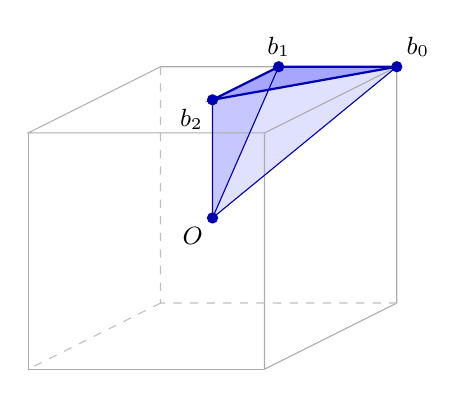
\begin{tikzpicture}[font=\small,scale=1.2]
	\coordinate (O) at (0,0);
	\coordinate (A) at (1.95,1.6);
	\coordinate (B) at (-.55,1.6);
	\coordinate (C) at (-1.95,.9);
	\coordinate (D) at (.55,.9);
	\coordinate (a) at (1.95,-.9);
	\coordinate (b) at (-.55,-.9);
	\coordinate (c) at (-1.95,-1.6);
	\coordinate (d) at (.55,-1.6);
	\coordinate (M) at (.7,1.6);
	\coordinate (F) at (0,1.25);
	\fill[blue!12] (O)--(A)--(M)--cycle;
	\fill[blue!22] (O)--(M)--(F)--cycle;
	\fill[blue!35] (A)--(M)--(F)--cycle;
	\draw[gray!65] (A)--(B)--(C)--(D)--cycle;
	\draw[gray!65] (A)--(a)--(d)--(D);
	\draw[gray!65] (C)--(c)--(d);
	\draw[gray!50,dashed] (B)--(b)--(a) (b)--(c);
	\draw[blue!70!black,thick] (A)--(M)--(F)--cycle;
	\draw[blue!70!black] (O)--(A) (O)--(M) (O)--(F);
	\foreach \p in {O,A,M,F} {\fill[blue!70!black] (\p) circle (1.7pt);}
	\node[below left] at (O) {\(O\)};
	\node[above right] at (A) {\(b_0\)};
	\node[above] at (M) {\(b_1\)};
	\node[below left] at (F) {\(b_2\)};
\end{tikzpicture}

	\caption[一面旗的中心链]{在立方体中选定顶点 \(b_0\)、包含它的棱及一个面，令 \(b_1\) 为该棱中点，\(b_2\) 为该面中心，\(O\) 为立方体中心。蓝色三角形是这面旗在边界上的区域，连接 \(O\) 后得到旗室的一部分。空间中的线段 \(b_0b_1,b_1b_2,b_2O\) 两两垂直；透视图中的投影角度不表示这些直角。}
	\label{g1:fig:polytope-flag-chamber}
\end{figure}

\begin{theorem}[旗室与壁反射]
	\label{g1:thm:regular-polytope-flag-chambers}
	设 \(P\) 为 \(n\ge2\) 维 Euclid 空间中的满维凸正多胞形，并把顶点平均点移到原点。固定一面旗 \(\Phi\)，令 \(b_i=c_{F_i}\)、\(0\le i\le n-1\)，且 \(b_n=0\)。则
	\[
		\mathcal C_\Phi=\left\{\sum_{i=0}^{n-1}t_i b_i:t_i\ge0\right\}
	\]
	是一个满维单纯锥。它是有限反射群 \(G(P)\) 的一个闭基本室；每个壁上的正交反射都属于 \(G(P)\)，这些 \(n\) 个反射生成 \(G(P)\)。各面旗的锥覆盖整个空间，内部两两不交，且 \(b_i-b_{i-1}\)、\(1\le i\le n\) 两两垂直。
\end{theorem}
\begin{proof}
	先建立几何分割，而不预设群由反射生成。在任意面中，以其中心连接边界的分割；从线段开始逐维归纳，可把每个面分成由它内部的面链中心生成的单纯形。中心在相对内部，保证这些单纯形覆盖整个面且只在公共子面相交。由此，\(\partial P\) 被各面旗的
	\[
		\operatorname{conv}\{b_0,\ldots,b_{n-1}\}
	\]
	分割。原点在内部，从原点出发的每条射线与边界恰交于一点；将这些边界单纯形沿射线张开，就得到所述锥的覆盖与内部不交性。\cref{g1:lem:regular-polytope-centers}的仿射无关性说明，每个锥都是满维单纯锥。

	每个这样的边界单纯形恰有一个只改变第 \(i\) 维面的相邻旗。这里需要核对“恰有一个”。若 \(i=0\)，\(F_1\) 是线段，只有两个端点可选。若 \(i\ge1\)，在 \(F_{i+1}\) 的仿射包络中以其内点为原点取极体。\cref{g1:prop:polar-face-duality}把它的 \((i-1)\) 维面 \(F_{i-1}\) 变成极体的一条棱，而介于 \(F_{i-1}\) 与 \(F_{i+1}\) 之间的 \(i\) 维面恰对应这条棱的两个端点。因此也只有两个选择，一个是原来的 \(F_i\)，另一个给出唯一相邻旗。

	旗传递提供一个变换 \(s_i\)，把基准旗送到上述相邻旗。它固定原点及全部 \(b_j\)、\(j\ne i\)，故逐点固定由这 \(n-1\) 个独立向量张成的壁超平面。它又不是恒等变换，因为改变了 \(F_i\)。非恒等正交变换若逐点固定一个超平面，就只能在其一维正交补上取负；所以 \(s_i\) 确为这个壁上的正交反射，且确实属于 \(G(P)\)。

	这些相邻关系把所有旗连通起来。具体说，在两个锥的内部选点，可用折线连接，并稍微选择折线的折点，使它不经过有限多个余维至少二的单纯形所在的子空间，也不沿任何壁行走。折线便依次穿过一串锥，每次只穿过一个公共壁。若已经到达 \(w\Phi\)，它的第 \(i\) 个相邻旗就是 \(ws_i\Phi\)。所以由 \(s_i\) 生成的群已在全部旗上传递。任意 \(g\in G(P)\) 与某个这样的乘积 \(w\) 送基准旗到同一面旗，\(w^{-1}g\) 固定旗，故由\cref{g1:lem:regular-polytope-centers}为恒等。于是这些反射生成整个 \(G(P)\)。

	还须核对这个锥就是反射超平面分割中的室。若群中某个反射的固定超平面穿过锥的内部，其反射像锥与原锥便有公共内点，因而是同一个旗锥；该反射于是固定这面旗，只能为恒等，矛盾。因此锥的内部不被其他反射超平面截开；它的各壁又都是反射超平面，故其内部恰是这个超平面排列的一个连通分支。由\cref{g1:prop:reflection-root-model}，取全部反射墙的两侧单位法向量，得到一个张成环境空间的有限约化实根系，其反射群就是 \(G(P)\)。\cref{g1:thm:reflection-chamber-fundamental}于是适用，给出闭基本室及每条轨道在其中的唯一代表。

	最后证明中心链的垂直性。保持任一面 \(F\) 的对称在其顶点上传递，所以各顶点到 \(c_F\) 等距；全部顶点到原点也等距。展开这两个平方距离之差，得到 \(\langle x,c_F\rangle\) 在 \(F\) 的顶点上为常数。取平均可知此常数为 \(\lVert c_F\rVert^2\)，所以 \(c_F\) 垂直于 \(F\) 的仿射包络的方向空间。对嵌套的面，\(b_j-b_{j-1}\) 因而垂直于 \(F_{j-1}\) 的方向空间；较早的每个差向量都在该方向空间内。因此这些差向量两两垂直。
\end{proof}

这个证明恢复了反射群与正多胞形之间的两项对应。群元素移动整面旗，墙反射只改变其中一层；闭基本室的边界则记录哪些局部对称固定了当前位置。反向构造轨道凸包时，面结构与旗传递就是需要验证的两项条件；下面在具体向量模型中计算它们。

\begin{proposition}[极对偶与共同的对称群]
	\label{g1:prop:regular-polar-duality}
	设 \(P\subset\mathbb R^n\) 为满维凸正多胞形，并把它的顶点平均点移到原点。则 \(P^\circ\) 也是正多胞形，而且 \(G(P)=G(P^\circ)\)。极面对偶按倒序对应两者的旗；三维中把 Schläfli 记号 \(\{p,q\}\) 变为 \(\{q,p\}\)。
\end{proposition}
\begin{proof}
	原点为内点，\cref{g1:prop:polar-face-duality}给出反转包含关系的面格双射，并交换互补维数。因此旗倒序后仍是完整的旗。对正交变换 \(Q\)，由内积不变性有 \((QP)^\circ=QP^\circ\)。由于 \(G(P)\) 中的元素固定原点，这说明 \(G(P)\) 保持极体，并通过旗的倒序对应在极体的旗上传递。

	为确定全对称群，先注意极体的顶点平均点也固定于 \(G(P)\)。这个群含有上一证明中的全部壁反射；它们的壁法向量线性无关，所以公共固定空间只有 \(\{0\}\)。故极体的顶点平均点也是原点，它的所有等距对称同样都是正交变换。再用双极公式，便得到反向包含 \(G(P^\circ)\subseteq G(P)\)。三维中，一个面的 \(p\) 条边对应极顶点的 \(p\) 条棱，一个顶点周围的 \(q\) 条棱对应一个 \(q\) 边形面，得到最后的记号变化。
\end{proof}

\begin{theorem}[三维凸正多面体的五种类型]
	\label{g1:thm:regular-three-classification}
	三维 Euclid 空间中，满维凸正多胞形在相似意义下恰有五种，即\cref{g1:tab:regular-three-polytopes}中的五个模型。
\end{theorem}
\begin{proof}
	设每个面为正 \(p\) 边形，每个顶点有 \(q\) 条棱经过。\cref{g1:lem:regular-polytope-centers}及\cref{g1:lem:vertex-figure-section}说明面与顶点图形都是正多边形，所以 \(p,q\ge3\)。取一面旗，沿用前一定理的 \(b_0,b_1,b_2\) 与壁反射 \(s_0,s_1,s_2\)。壁 \(0\) 和壁 \(1\) 的公共射线经过面中心 \(b_2\)；在垂直于这条射线的面平面内，旗三角形正是正 \(p\) 边形的一半中心扇形，故两壁在室内的夹角为 \(\pi/p\)。同样，在垂直于顶点射线 \(\mathbb R_{\ge0}b_0\) 的顶点图形中，壁 \(1\) 与壁 \(2\) 的室内夹角为 \(\pi/q\)。

	另外两个壁垂直。具体令 \(u=b_0-b_1\)、\(v=b_1-b_2\)、\(w=b_2\)，则三者两两垂直，且
	\[
		b_0=u+v+w,\qquad b_1=v+w,\qquad b_2=w.
	\]
	壁 \(0\) 张成为 \(\operatorname{span}\{v,w\}\)，其法向沿 \(u\)；壁 \(2\) 张成为 \(\operatorname{span}\{u,v+w\}\)，其法向垂直于 \(u\)。所以二者夹角为 \(\pi/2\)。

	取三个壁的朝室内的单位法向量。按式\eqref{g1:eq:reflection-angle-product}中的反射角约定，它们的 Gram 矩阵为
	\[
		M_{p,q}=
		\begin{pmatrix}
			1&-\cos(\pi/p)&0\\
			-\cos(\pi/p)&1&-\cos(\pi/q)\\
			0&-\cos(\pi/q)&1
		\end{pmatrix}.
	\]
	三个法向量独立，故此矩阵正定，特别地
	\[
		0<\det M_{p,q}
		=1-\cos^2(\pi/p)-\cos^2(\pi/q).
	\]
	因 \(0<\pi/p,\pi/q<\pi/2\)，该不等式等价于
	\begin{equation}
		\label{g1:eq:regular-three-pq-bound}
		\frac1p+\frac1q>\frac12.
	\end{equation}
	若 \(p,q\) 都至少为 \(4\)，左边至多为 \(1/2\)，不可能。因此至少一个为 \(3\)，另一个只能为 \(3,4,5\)。恰得到 \((3,3),(4,3),(3,4),(5,3),(3,5)\)，各型的存在已由前面构造证明。

	还须证明同一型不会给出不相似的模型。相同 \(p,q\) 给出相同的正定 Gram 矩阵，因此两组有序单位法向量可由一个正交变换对应；把一个模型旋转或反射后，其三个壁及选定基本室就与另一个重合。这面旗的顶点射线是壁 \(1\) 与壁 \(2\) 的交在室内的一条边。再作一次正比例缩放，可以使两个基准顶点重合。三壁反射此时逐个相同，而\cref{g1:thm:regular-polytope-flag-chambers}已证明它们生成整个对称群。顶点传递说明全部顶点恰为基准顶点的群轨道，所以两份顶点集、进而两份凸包完全相同。这就证明了相似唯一性。
\end{proof}

\subsection{正二十四胞体}
\label{g1:subsec:E03:05}

单纯形、立方体和交叉多面体在每个维数都存在。在四维中，\(D_4\) 的最短向量给出这三族之外的一个模型：前面格堆积中负责接触关系的向量，现在直接用作凸包的顶点。

\begin{proposition}[正二十四胞体]
	\label{g1:prop:regular-24-cell}
	在标准Euclid 空间 \(\mathbb R^4\) 中令
	\[
		R=\{\pm e_i\pm e_j:1\le i<j\le4\},\qquad
		P_{24}=\operatorname{conv}R.
	\]
	则 \(P_{24}\) 是一个有 \(24\) 个顶点、\(24\) 个三维余维一的面的正多胞形。这些三维面均为边长 \(\sqrt2\) 的正八面体；它们的支撑法向量分成
	\begin{equation}
		\label{g1:eq:24-cell-normals}
		N_{24}=\{\pm e_i:1\le i\le4\}
		\ \cup\ 
		\left\{\frac12(\varepsilon_1,\varepsilon_2,\varepsilon_3,\varepsilon_4):
		\varepsilon_i\in\{1,-1\}\right\},
	\end{equation}
	且每个支撑值都为 \(1\)。全对称群阶为 \(1152\)，并且 \(P_{24}\) 自对偶。
\end{proposition}
\begin{proof}
	先确定凸包与全部余维一的面。令
	\[
		Q=\{x\in\mathbb R^4:|x_i|\le1\ (1\le i\le4),\ 
		\sum_{i=1}^4|x_i|\le2\}.
	\]
	最后一个条件等价于对全部十六种符号选择要求 \(\sum_i\varepsilon_ix_i\le2\)，故 \(Q\) 是有界多面体。显然 \(R\subseteq Q\)。反过来，若 \(x\in Q\) 满足 \(\sum_i|x_i|<2\)，绝对值限制中至少有一个坐标尚未固定在 \(\pm1\)；沿此坐标作足够小的正负扰动仍在 \(Q\) 中，故 \(x\) 不是顶点。若 \(\sum_i|x_i|=2\) 且至少两个非零坐标的绝对值严格介于 \(0\) 与 \(1\) 之间，则可让这两个绝对值一增一减，仍得到非平凡线段分解。若这样的坐标只有一个，其绝对值应为 \(2\) 减去若干个 \(1\)，不可能严格介于 \(0\) 与 \(1\) 之间。因此 \(\operatorname{Vert}Q\subseteq R\)。\cref{g1:thm:polytope-hv}及 \(R\subseteq Q\) 给出 \(Q=\operatorname{conv}R=P_{24}\)。此外 \(R\) 各点同在平方半径为 \(2\) 的球面上，各点均被自身在这个凸包上唯一暴露，确实都是顶点。

	由这份半空间表示，候选支撑面正是式\eqref{g1:eq:24-cell-normals}给出的二十四个限制。对法向量 \(e_i\)，取等号的顶点是
	\[
		e_i\pm e_j\qquad(j\ne i).
	\]
	以 \(e_i\) 为中心平移后，它们是三维正交补中的六个单位坐标向量，故生成正八面体。法向量 \(-e_i\) 同理。

	对 \(n=\tfrac12(\varepsilon_1,\ldots,\varepsilon_4)\)，取等号的六个顶点为
	\[
		\varepsilon_ie_i+\varepsilon_je_j\qquad(1\le i<j\le4).
	\]
	它们平均为 \(n\)。互补的两对指标给出关于 \(n\) 相反的两个点；从三个相反点对中各取一个，减去 \(n\) 后得到三个两两垂直的单位向量。例如所有 \(\varepsilon_i=1\) 时可取
	\[
		\frac12(1,1,-1,-1),\quad
		\frac12(1,-1,1,-1),\quad
		\frac12(1,-1,-1,1).
	\]
	改变坐标符号保持这些内积。因此这一类面也都是正八面体。每条列出的限制都真正给出三维面；而有限半空间交的余维一的面必来自某条限制，所以二十四个面已经穷尽。

	现在核验旗传递。全部坐标符号改变和坐标置换保持 \(R\)，在上述八个坐标法向量间传递，也在十六个半整数法向量间传递。为把两类面联系起来，取
	\[
		T=\frac12
		\begin{pmatrix}
			1&1&1&1\\
			1&1&-1&-1\\
			1&-1&1&-1\\
			1&-1&-1&1
		\end{pmatrix}.
	\]
	它的各列正交且长为 \(1\)，所以 \(T\) 正交。两列的和或差恰有两个坐标为 \(\pm1\)，其余为零，所以 \(T\) 置换 \(R\)。此外 \(Te_1=(1,1,1,1)/2\)，故它把一个坐标法向面送到一个半整数法向面。由此，已构造的对称在全部二十四个三维面上传递。

	固定面 \(x_1=1\) 时，任意改变后三个坐标的符号及置换后三个坐标，仍保持 \(P_{24}\)，并在该面上实现正八面体的全部 \(48\) 个对称。因此它的稳定子在该面的旗上传递。先移动一面旗所属的三维面，再在该面内移动旗，就得到 \(P_{24}\) 的旗传递。每个三维面有 \(48\) 面旗，全部旗数为 \(24\cdot48=1152\)，由\cref{g1:lem:regular-polytope-centers}等于全对称群阶。

	最后给出自对偶的实际相似变换。由已经核实且不可省略的支撑面表示，极体为 \(P_{24}^\circ=\operatorname{conv}N_{24}\)。令
	\[
		K=
		\begin{pmatrix}
			1&1&0&0\\
			1&-1&0&0\\
			0&0&1&1\\
			0&0&1&-1
		\end{pmatrix},\qquad K^{\mathsf T}K=2I.
	\]
	它把八个 \(\pm e_i\) 送到支撑在前两个或后两个坐标上的八个根向量。对于半整数点，
	\[
		K\frac{(\varepsilon_1,\varepsilon_2,\varepsilon_3,\varepsilon_4)}2
		=\left(\frac{\varepsilon_1+\varepsilon_2}2,
		\frac{\varepsilon_1-\varepsilon_2}2,
		\frac{\varepsilon_3+\varepsilon_4}2,
		\frac{\varepsilon_3-\varepsilon_4}2\right),
	\]
	其前两个坐标恰有一个为 \(\pm1\)，后两个坐标也恰有一个为 \(\pm1\)，给出其余十六个根向量。因此 \(KN_{24}=R\)，即 \(KP_{24}^\circ=P_{24}\)。矩阵 \(K\) 是正交变换后接比例 \(\sqrt2\) 的相似变换，故确得几何自对偶。
\end{proof}

这个模型称为\term[zhengershisibaoti]{正二十四胞体}[regular 24-cell]。\symidx{\(P_{24}\)：正二十四胞体}四维多胞形的三维余维一的面通常称为\term[bao]{胞}[cell]；这里的“二十四”数的就是这些正八面体胞。它既不是四维立方体，也不是四维交叉多面体：三者的顶点数分别为 \(24,16,8\)，胞数分别为 \(24,8,16\)。正二十四胞体与根系共享同一组向量坐标，因而它的顶点、面与对称变换都可以从这份数据中计算。

\ProseParagraphBreak

三维分类之所以能在上面完成，是因为旗室只有三个壁，且唯一需要限制的两个整数已由式\eqref{g1:eq:regular-three-pq-bound}穷尽。高维完整分类还需要对任意旗室的全部相邻壁角作正定性分析，证明相应图的穷尽性，并由允许的壁系统恢复各个多胞形。本节的三族任意维模型与四维正二十四胞体展示了反射、旗和极体如何共同计算。

\section{凸多面体的整体刚性}
\label{g1:sec:E04}

把硬纸板裁成若干多边形，再沿规定的边粘合，面本身的形状并没有告诉我们相邻两面应当张开多少。一般的铰接结构确实可能活动。Cauchy 定理说明，若这些面已经围成一个三维凸多面体，那么各面的形状和粘合关系便共同确定了整个空间形状。本节把这一结论分成两个问题：在一个顶点附近，二面角的改变必须怎样交替；在整个球面图上，这种交替是否可能处处发生。

\ProseParagraphBreak

证明使用第3章的多面体与面格、第10.1节的球面短弧和余弦公式，以及有限平面图的 Euler 计数。球面臂引理采用 Schoenberg--Zaremba 的归纳思路\cite[第3节，第1070--1071页]{SchoenbergZaremba1967CauchyLemma}，在归纳步骤中核对端点转动时保持凸性的条件。Cauchy 定理的球面链接路线也可见\cite[第14章，第95--96页]{AignerZiegler2018Proofs}。

\subsection{面度量、组合对应与刚性问题}
\label{g1:subsec:E04:01}

本节的三维凸多面体，是 \(\mathbb R^3\) 中有非空内部的有界凸多面体；由\cref{g1:thm:polytope-hv}，它也就是一个三维凸多胞形。所说的面、棱、顶点均指\cref{g1:def:polytope-face}中的实际面，不把同一平面内人为添加的分割线当作棱。特别地，两个相邻二维面不共面，它们的内二面角属于 \((0,\pi)\)。

\begin{definition}[对应面全等的数据]\label{g1:def:cauchy-face-data}
	设 \(P,P'\subset\mathbb R^3\) 是有非空内部的凸多胞形。其面格之间保持包含关系的同构 \(\varphi\)，称为一个\term[duomianthizuheduiying]{组合对应}[combinatorial correspondence]。若对每个二维面 \(F\subset P\)，都有所在平面之间的 Euclid 等距映射，将 \(F\) 的每个顶点 \(v\) 送到 \(\varphi(v)\)，就说这一对应的各面全等。
\end{definition}

组合对应规定哪些顶点、棱和面彼此关联；面全等则规定每个平面多边形的完整形状，包括面内的角和对角线。单有棱长相等，对一般多边形面并不够。各面之间的等距映射也尚未被假定为同一个空间运动的限制；它们能否由一个空间等距映射同时实现，正是要证明的问题。

\ProseParagraphBreak

对一条棱 \(e\)，在其相对内部取点，用垂直于棱的平面截开多面体，得到一个平面凸角。这个凸角在多面体内部的角度记为 \(\delta_e\)，称为\term[neiermianjiao]{内二面角}[interior dihedral angle]。若相邻面的单位外法向量为 \(n_1,n_2\)，则
\begin{equation}\label{g1:eq:interior-dihedral-normal-angle}
	\delta_e=\pi-\arccos\langle n_1,n_2\rangle.
\end{equation}
后面给棱标号时，一律比较这个内部角，而不是外法向量之间的角。定理中的\term[duomianthizhengtiqixing]{整体刚性}[global rigidity]，是指任意两组满足这些面数据的凸实现都由一个 Euclid 空间等距映射联系；它比排除某条连续活动路径的说法更强。

\subsection{凸多面体的球面链接}
\label{g1:subsec:E04:02}

围绕顶点画一个很小的球，原来聚在顶点处的棱变成球面上的点，面内的夹角变成连接这些点的短弧。这样便能在一个二维球面多边形上同时记录该顶点附近的面角与二面角。

\begin{definition}[严格凸球面多边形]\label{g1:def:cauchy-spherical-polygon}
	单位球面 \(S^2\) 上依次给定 \(m\ge3\) 个点。若它们同处一个开半球，且从球心向该半球内一个仿射平面的中心投影，将依次连接的短大圆弧送到一个各内角均小于 \(\pi\) 的平面凸多边形，就称这些短弧围成一个\term[yangeqiumentubianxing]{严格凸球面多边形}[strictly convex spherical polygon]。球面角取两条边的切向量所夹的内部角。
\end{definition}

中心投影保持短弧与线段及其相交、包含关系，所以这个定义与所选投影平面无关。边长和角度仍须在球面上测量，不能用投影图中的 Euclid 长度和角代替。

\begin{proposition}[链接的两种角度对应]\label{g1:prop:vertex-spherical-link}
	设 \(P\subset\mathbb R^3\) 是三维凸多胞形，\(v\) 是其顶点。充分小的 \(\varepsilon>0\) 使
	\[
		L_v=\{u\in S^2:v+\varepsilon u\in P\}
	\]
	成为严格凸球面多边形，而且与这一充分小的 \(\varepsilon\) 无关。它的顶点对应于经过 \(v\) 的棱，边对应于经过 \(v\) 的二维面；每条链接边的长度等于相应面在 \(v\) 处的平面内角，每个链接内角等于相应棱的内二面角。
\end{proposition}
\begin{proof}
	将 \(P\) 写成其各面支撑半空间的交。在 \(v\) 处取等号的那些不等式，定义一个以原点为顶点的锥
	\[
		C_v=\{w:\langle n_F,w\rangle\le0\text{，其中 }F\text{ 遍历含 }v\text{ 的二维面}\}.
	\]
	其余不等式在 \(v\) 处有严格余量；因其只有有限个，可取 \(\varepsilon\) 足够小，使球 \(B_\varepsilon(v)\) 内这些不等式均自动满足。因此在该球内 \(P\) 与 \(v+C_v\) 相同，且 \(L_v=C_v\cap S^2\)。锥有三维内部，其极射线是含 \(v\) 的棱的方向，二维锥面是含 \(v\) 的二维面的方向；这也可由各面的取等号条件直接核对。

	由顶点的极端性，\(v\) 不在其他顶点的凸包内。严格分离 \(v\) 与这一紧凸包，可得一个向量 \(a\)，使 \(\langle a,w-v\rangle>0\) 对每个其他顶点 \(w\) 成立。锥由这些方向生成，所以 \(\langle a,u\rangle>0\) 对 \(u\in L_v\) 成立。故链接包含在一个开半球内。中心投影将其送到锥的一个有界凸截面；实际的棱和面给出该截面的全部顶点和边，没有人为加入的平角。

	相邻棱的单位方向记为 \(u_i,u_{i+1}\)。它们位于同一个面内，且在该面中夹成小于 \(\pi\) 的角 \(\beta_i\)。球面短弧的长度为
	\[
		d_{S^2}(u_i,u_{i+1})=\arccos\langle u_i,u_{i+1}\rangle=\beta_i.
	\]
	再看链接顶点 \(u_i\)。球面的切平面是 \(u_i^\perp\)，其两条边的切线分别是两个相邻面平面与 \(u_i^\perp\) 的交线；朝向链接内部的两条射线，恰是垂直于原棱的截面中朝向两个面的射线。球面内部与多面体内部选取同一个凸角，因而此处的球面内角就是 \(\delta_{e_i}\)。式\eqref{g1:eq:interior-dihedral-normal-angle}也给出同一结论。
\end{proof}

这个球面多边形称为顶点的\term[dingdianqiumianlianjie]{球面链接}[spherical link]。若 \(P,P'\) 的对应面全等，则对应链接的边长逐一相等；可能不同的只剩链接的内角，也就是原多面体的二面角。\cref{g1:fig:vertex-link-dihedral}分别画出一个链接模型和垂棱截面的内部角约定。

\begin{figure}[htbp]
	\centering
	% !TeX root = ../Book1.tex
\begin{tikzpicture}[>=latex,line cap=round,line join=round,font=\small]
	\begin{scope}[x={(1.65cm,-0.48cm)},y={(-1.15cm,-0.83cm)},z={(0cm,1.65cm)}]
		\fill[blue!12] (1,0,0) -- plot[domain=0:90,samples=30,variable=\t] ({cos(\t)},{sin(\t)},0) -- plot[domain=0:90,samples=30,variable=\t] (0,{cos(\t)},{sin(\t)}) -- plot[domain=0:90,samples=30,variable=\t] ({sin(\t)},0,{cos(\t)}) -- cycle;
		\draw[gray,dashed] (0,0,0) -- (1.4,0,0);
		\draw[gray,dashed] (0,0,0) -- (0,1.4,0);
		\draw[gray,dashed] (0,0,0) -- (0,0,1.3);
		\draw[thick,blue!65!black] plot[domain=0:90,samples=30,variable=\t] ({cos(\t)},{sin(\t)},0);
		\draw[thick,blue!65!black] plot[domain=0:90,samples=30,variable=\t] (0,{cos(\t)},{sin(\t)});
		\draw[thick,blue!65!black] plot[domain=0:90,samples=30,variable=\t] ({sin(\t)},0,{cos(\t)});
		\fill (0,0,0) circle (1.2pt) node[below] {$v$};
		\fill (1,0,0) circle (1.3pt) node[right] {$u_1$};
		\fill (0,1,0) circle (1.3pt) node[left] {$u_2$};
		\fill (0,0,1) circle (1.3pt) node[above right] {$u_3$};
	\end{scope}
	\node at (0,-1.8) {顶点与球面链接};
	\begin{scope}[shift={(6.3cm,0cm)}]
		\fill[blue!12] (0,0) -- (1.8,0) arc[start angle=0,end angle=65,radius=1.8] -- cycle;
		\draw[thick] (0,0) -- (2,0) node[right] {$F_1$};
		\draw[thick] (0,0) -- (65:2) node[above right] {$F_2$};
		\draw (0.55,0) arc[start angle=0,end angle=65,radius=0.55];
		\node at (32.5:0.82) {$\delta$};
		\draw[->,thick,red!65!black] (0,0) -- (-90:1.35) node[right] {$n_1$};
		\draw[->,thick,red!65!black] (0,0) -- (155:1.35) node[above left] {$n_2$};
		\draw[red!65!black] (155:0.66) arc[start angle=155,end angle=270,radius=0.66];
		\node[red!65!black] at (212.5:1.02) {$\pi-\delta$};
		\fill (0,0) circle (1.2pt);
	\end{scope}
	\node at (6.7,-1.8) {垂棱截面的角度约定};
\end{tikzpicture}

	\caption[球面链接与内二面角]{左图为立方体顶点的单位球面链接，三条链接边均长 \(\pi/2\)；原顶点到三个链接顶点的线段表示棱的方向。右图在垂棱平面中比较内二面角 \(\delta\) 与外法向量夹角 \(\pi-\delta\)。}
	\label{g1:fig:vertex-link-dihedral}
\end{figure}

\subsection{Cauchy 变号引理}
\label{g1:subsec:E04:03}

先把一个球面多边形的一条边留作可变化的开口。其余边长保持不变，并把沿途的内部角都张大时，开口应当变长。困难在于任意选择的逐角转动可能破坏凸性；下面证明\term[qiumianbiyinli]{球面臂引理}[Cauchy\textquotesingle s spherical arm lemma]；归纳中在第一次出现平角时缩短多边形，而不继续使用已经失去凸性的图形。

\begin{lemma}[球面臂引理]\label{g1:lem:spherical-cauchy-arm}
	设 \(A=(a_1,\ldots,a_n)\)、\(B=(b_1,\ldots,b_n)\) 是单位球面上的严格凸多边形，\(n\ge3\)。设其内部角分别为 \(\alpha_i,\beta_i\)，并且
	\[
		d(a_i,a_{i+1})=d(b_i,b_{i+1})\quad(1\le i<n),\qquad
		\alpha_i\le\beta_i\quad(2\le i<n).
	\]
	这里 \(d\) 是球面短弧距离。则
	\[
		d(a_1,a_n)\le d(b_1,b_n),
	\]
	且等号成立当且仅当 \(\alpha_i=\beta_i\) 对所有 \(2\le i<n\) 成立。
\end{lemma}
\begin{proof}
	按 \(n\) 归纳。三角形中，两边长 \(r,s\in(0,\pi)\) 固定，夹角为 \(t\in(0,\pi)\) 时，球面余弦公式给出对边长 \(c\)：
	\[
		\cos c=\cos r\cos s+\sin r\sin s\cos t.
	\]
	由于 \(\sin r\sin s>0\)，而 \(\cos\) 在 \((0,\pi)\) 上严格递减，\(c\) 随 \(t\) 严格增加。这同时证明 \(n=3\) 的不等式和等号条件。

	设 \(n>3\)，且结论对少于 \(n\) 个顶点的多边形成立。如果某个 \(2\le j<n\) 满足 \(\alpha_j=\beta_j\)，则三角形 \(a_{j-1}a_ja_{j+1}\) 与 \(b_{j-1}b_jb_{j+1}\) 由两边及夹角全等。在两个多边形中删去相应顶点，改用对角线连接邻点，就得到两个严格凸的 \((n-1)\) 边形。新边长度相等；两个相邻内部角分别减去全等三角形中相同的角，其比较方向不变，任何原有的严格不等式也保留。归纳假设便给出所需结论及等号条件。

	以下只剩所有 \(\alpha_i<\beta_i\)、\(2\le i<n\) 的情形。固定 \(a_1,\ldots,a_{n-1}\)，令最后一点 \(x\) 在以 \(a_{n-1}\) 为球面中心、半径 \(d(a_{n-1},a_n)\) 的圆上转动，使顶点 \(a_{n-1}\) 的内部角 \(t\) 从 \(\alpha_{n-1}\) 增加到 \(\beta_{n-1}<\pi\)。在原多边形内，对角线 \(a_{n-1}a_1\) 与 \(a_{n-1}a_{n-2}\) 的夹角记为 \(\theta\)，有 \(0<\theta<\alpha_{n-1}\)。三角形 \(a_1a_{n-1}x\) 在 \(a_{n-1}\) 的角为 \(t-\theta\in(0,\pi)\)。因此该三角形始终非退化，\(d(a_1,x)\) 严格增加，且始终属于 \((0,\pi)\)。它也保证移动点 \(x\) 处的角不可能先变成平角。

	下面核对转动中可能发生的第一种退化。只要多边形严格凸，各有向边所在大圆的左闭半球就包含全部顶点。取使其左侧为正的单位向量
	\[
		u=\frac{a_1\times a_2}{|a_1\times a_2|},\qquad
		w=\frac{a_2\times a_3}{|a_2\times a_3|}.
	\]
	向量 \(u+w\) 与所有固定顶点中除 \(a_2\) 以外的点内积严格为正，与 \(a_2\) 内积为零，与移动点的内积非负；这些关系在第一次退化的极限位置仍成立。如果极限顶点不再同处某个开半球，严格分离定理就说明原点属于它们的凸包。与 \(u+w\) 配对后，凸组合只能使用 \(a_2\) 和移动点，故后者必须是 \(-a_2\)。当 \(n=4\) 时，这会使 \(a_{n-1}\) 处的角等于 \(\pi\)，与 \(t\le\beta_{n-1}<\pi\) 矛盾；当 \(n>4\) 时，固定边 \(a_{n-2}a_{n-1}\) 的正侧严格包含 \(a_2\)，不可能同时包含 \(-a_2\)。故极限仍处于某个开半球，不会因出现对径点而丢失短弧的含义。

	在这个半球内作中心投影，凸性退化便是普通凸多边形的退化。移动点与 \(a_1,a_{n-1}\) 始终组成非退化三角形，且它与固定的其他顶点分处对角线 \(a_1a_{n-1}\) 两侧，所以不会碰到其他顶点。固定的各内部角 \(a_2,\ldots,a_{n-2}\) 没有变化，\(a_{n-1}\) 处的角仍小于 \(\pi\)，移动点处也没有平角。因此若凸性先到边界，只能是 \(a_1\) 处的角变为 \(\pi\)；此时 \(a_1\) 位于从 \(a_2\) 到移动点 \(x_*\) 的短弧内部，且
	\begin{equation}\label{g1:eq:spherical-arm-flat-end}
		d(a_2,x_*)=d(a_2,a_1)+d(a_1,x_*).
	\end{equation}
	删去这个平角顶点，剩下的多边形仍严格凸。这里中心投影也说明了 \(a_1\) 在短弧中的次序；不能把球面上经过对径点的长弧用于这个等式。

	如果直到 \(t=\beta_{n-1}\) 都未出现平角，则转动后的多边形 \(A_*\) 与 \(B\) 在 \(n-1\) 处有相同内部角。对它们使用前面的删顶点步骤与归纳假设，得到
	\[
		d(b_1,b_n)\ge d(a_1,x_*)>d(a_1,a_n).
	\]
	如果在某个 \(t\le\beta_{n-1}\) 先于或恰在终点出现平角，则比较严格凸的多边形
	\[
		(a_2,a_3,\ldots,a_{n-1},x_*),\qquad
		(b_2,b_3,\ldots,b_{n-1},b_n).
	\]
	它们沿途各边长相同，各内部角满足归纳假设，故 \(d(b_2,b_n)\ge d(a_2,x_*)\)。再用距离的三角不等式和\eqref{g1:eq:spherical-arm-flat-end}，得到
	\begin{align*}
		d(b_1,b_n)
		&\ge d(b_2,b_n)-d(b_1,b_2)\\
		&\ge d(a_2,x_*)-d(a_1,a_2)
		=d(a_1,x_*)>d(a_1,a_n).
	\end{align*}
	两种情形均为严格不等式。结合有相等内部角时的归纳步骤，证明了全部结论。
\end{proof}

由臂引理可以得到\term[qiumianCauchybianhaoyinli]{球面 Cauchy 变号引理}[Cauchy\textquotesingle s spherical sign-change lemma]，它限制了相应内角差在边界上的排列。

\begin{lemma}[球面 Cauchy 变号引理]\label{g1:lem:spherical-cauchy-sign}
	设两个严格凸球面 \(m\) 边形具有逐一相等的相应边长，其相应内部角为 \(\alpha_i,\beta_i\)。按循环次序给非零差 \(\beta_i-\alpha_i\) 标记正负号，并略去零差。如果存在非零差，则这些符号在一周内至少改变四次。
\end{lemma}
\begin{proof}
	循环符号列的变号次数为偶数。若没有变号，则所有非零差同号；交换两个多边形后可设它们均为正。选一条不以某个正号顶点为端点的边作开口，球面臂引理说明该边在第二个多边形中严格变长，与相应边长相等矛盾。

	若恰有两次变号，正号与负号便分别位于两个连续块中，零差允许夹在其中。可在两个符号块之间各选一条边，并连接这两条边的中点 \(M,N\)；在第二个多边形中连接相应中点 \(M',N'\)。由于两条边不同，这些连接都是多边形内部的短弧，分别将两个多边形切成两个严格凸多边形。沿正号一侧从 \(M\) 到 \(N\) 的链，相应边长相等，全部中间角不减且至少一个增加，故臂引理给出 \(d(M',N')>d(M,N)\)。沿负号一侧反向比较，同一引理却给出 \(d(M',N')<d(M,N)\)。两者矛盾。

	所以零次与两次变号均不可能，只能至少有四次。
\end{proof}

变号引理直接比较两个已经给定的凸多边形。臂引理中的转动用于归纳证明，并在失去严格凸性之前停止。

\subsection{Cauchy 凸多面体刚性定理}
\label{g1:subsec:E04:04}

一个顶点的链接要求至少四次变号，整个球面的 Euler 计数却不允许每个有关顶点都满足这个要求。先把后一件事单独证明。

\begin{lemma}[球面图的变号计数]\label{g1:lem:spherical-graph-sign-count}
	设有限简单图嵌入球面，每条边标为正或负，且至少有一条边。则存在一个与边关联的顶点，使围绕它的循环符号列至多变号两次。
\end{lemma}
\begin{proof}
	反设每个非孤立顶点至少有四次变号。取含边的一个连通分支，记其顶点数、边数、面数为 \(V,E,F\)，每个顶点的度至少为四。沿各面边界计数时，同一条桥的两侧分别出现，边界顶点也可重复；以下的边界长度均按这种出现次数计算。

	该连通球面图满足 \(V-E+F=2\)。例如不断删去圈上的边，每次边数和面数各减一，最终成为一棵树；树有 \(E=V-1\) 且补集只有一个面，这就证明公式。这个过程允许面边界重复经过桥，无须假定原图的每个面由简单圈围成。

	每个面边界的长度 \(k\) 至少为三：图中没有自环或平行边，而长度二的边界若只是同一条桥往返，便迫使整个连通分支只有这一条边，与顶点度数至少四矛盾。长度为 \(k\) 的循环正负列，其变号数 \(s\) 为偶数且不超过 \(k\)，因而
	\[
		s\le2(k-2).
	\]
	对 \(k=3\) 这是 \(s\le2\)，对 \(k\ge4\) 则由 \(s\le k\le2k-4\) 得到。

	一个顶点处两条相邻边之间的扇区，同时也是某个面边界的一个角。故从顶点和面两边所数的变号总数 \(S\) 相同。每条边在各面边界中共出现两次，于是
	\[
		4V\le S\le\sum_{\text{各面}}2(k-2)=4E-4F=4V-8,
	\]
	矛盾。变号次数为偶数，所以至少一个有关顶点的变号次数只能为零或二。
\end{proof}

把上述两个变号引理用于顶点链接，就得到\term[Cauchytuduomiantigangxing]{Cauchy 凸多面体刚性定理}[Cauchy\textquotesingle s rigidity theorem for convex polyhedra]。\footnote{Augustin-Louis Cauchy，1789--1857，法国数学家，在实分析、复分析及置换群理论中作出基础贡献。}

\begin{theorem}[Cauchy 凸多面体刚性定理]\label{g1:thm:cauchy-convex-rigidity}
	设 \(P,P'\subset\mathbb R^3\) 是有非空内部的凸多胞形，\(\varphi\) 是其面格的同构。若每个二维面与其对应面按 \(\varphi\) 规定的顶点对应全等，则存在 Euclid 空间等距映射 \(T\)，使
	\[
		T(P)=P',\qquad T(F)=\varphi(F)
	\]
	对每个面 \(F\) 成立。特别地，所有相应棱的内二面角相等。
\end{theorem}
\begin{proof}
	先证明二面角相等。给 \(P\) 的棱 \(e\) 按 \(\delta'_{\varphi(e)}-\delta_e\) 的符号标记，零差的棱暂不标记。在 \(P\) 内取点 \(o\)，从 \(o\) 向单位球面作径向投影。每条射线与边界恰交一点，所以边界到球面的投影是连续双射；边界紧而球面 Hausdorff，故它是同胚。于是去掉零差棱及孤立顶点后，留下的是一个嵌入球面的有限简单带符号图。

	若这个图非空，球面图变号计数引理给出某个顶点，使其非零棱号在循环次序中至多改变两次。在该顶点及对应顶点取单位球面链接。由\cref{g1:prop:vertex-spherical-link}，对应链接的边长相等，内部角差恰为各关联棱的二面角差。其循环次序由面格关联确定，允许整体反向；反向不改变变号次数。球面 Cauchy 变号引理却要求至少四次，矛盾。故带符号图为空，全部相应二面角相等。

	再说明这些角如何决定空间中的整体位置。先用一个空间等距映射使某一对对应面 \(F_0,F'_0\) 重合，并使两多面体位于该面平面的同一闭半空间。一个平面等距映射有两个空间等距延拓，恰可利用这两个选择确定朝内的一侧。

	设某一对对应面 \(F,F'\) 已重合，且朝内半空间也相同。沿其中一条棱 \(e\) 看相邻面 \(G,G'\)。在垂棱截面中，面 \(F\) 内朝向其内部的射线已经固定，多面体在 \(F\) 的哪一侧也已固定。相同的内部角 \(\delta_e\in(0,\pi)\) 因而唯一确定朝向 \(G\) 内部的射线。故 \(G,G'\) 位于同一平面和棱的同一侧。它们的给定面全等又固定棱的两个端点，在这一侧只有一种放置，遂使所有对应顶点重合。新面朝内的半空间也一致，因为两者都包含先前的面 \(F\)，而 \(F\) 不与新面共面。

	最后，面邻接图连通。确实，球面上两个面内点可以用一条避开有限顶点、与各棱横截的分段短弧连接；沿途依次经过相邻面。于是前一步能传到所有二维面，使全部对应顶点重合。多胞形是其顶点的凸包，故两多胞形重合，并实现规定的全部面对应。撤销最初的归一化，便得到所需的 \(T\)。
\end{proof}

定理比较任意两种凸实现，所以即使没有给出它们之间的连续变形，也能断定其全等。证明中，凸性分别保证了严格凸的球面链接、内部角的单值选择以及由一个已固定面向相邻面的唯一传播；球面拓扑则负责排除处处至少四次变号。

\subsection{凸性条件与光滑曲面刚性的比较}
\label{g1:subsec:E04:05}

删去凸性后，相同的三角形面及相同的粘合关系就可能给出不同的嵌入形状。下面将用同一组边长和三角形面，分别拼出一个凸的嵌入形状与一个非凸的嵌入形状。

\begin{example}[三角双锥与内凹实现]\label{g1:exm:cauchy-nonconvex-pair}
	在平面 \(z=0\) 中取以原点为重心的正三角形 \(ABC\)，并取
	\[
		U=(0,0,2),\qquad L=(0,0,-1),\qquad L_+=(0,0,1).
	\]
	顶点为 \(A,B,C,U,L\) 的凸双锥有六个三角形面。保留上面的三个面 \(UAB,UBC,UCA\)，将下面三个面关于 \(z=0\) 反射，改用 \(L_+AB,L_+BC,L_+CA\)。相应三角形全等，抽象的顶点、棱和面关联也完全相同。

	\ProseParagraphBreak

	为核对这六个面确实给出嵌入的闭曲面，在底三角形上令 \(h\) 为重心处值为一、边界值为零，并在重心到三条边形成的三个三角形上分别仿射的函数。两个三角锥侧面分别是 \(z=2h(x,y)\) 与 \(z=h(x,y)\) 的图像；在底三角形内部有 \(2h>h\)，它们只在边界粘合，故没有自交。其围成的区域却不凸：它包含 \(A,B,C\)，却不包含三者的重心 \((0,0,0)\)。

	\ProseParagraphBreak

	若底面积为 \(S\)，原凸双锥体积为 \(S(2+1)/3=S\)，内凹区域的体积为 \(S(2-1)/3=S/3\)，所以两者不可能全等。这证明了删去凸性后全局结论会失败；它本身并未构造一条保持面形的连续活动路径。
\end{example}

光滑曲面中的度量数据还须另作区分。第一基本形式记录内在长度，第二基本形式记录法向弯曲。在矩形 \((-\pi/4,\pi/4)\times(-1,1)\) 上，两个嵌入
\[
	X(u,v)=(u,v,0),\qquad Y(u,v)=(\cos u,\sin u,v)
\]
都诱导度量 \(\mathrm du^2+\mathrm dv^2\)，但一个像在平面内，另一个像在圆柱面内，不能由空间等距映射联系。相同的第一基本形式因而不能独自给出一般曲面片的空间刚性。

\ProseParagraphBreak

第8章的曲面基本定理使用第一、第二基本形式及其相容方程，处理局部重建与刚性变换意义下的唯一性。本节则从有限个平面面的完整度量和组合对应出发，利用整个凸边界的球面拓扑确定二面角。若要从这一有限组合证明过渡到仅由内在度量确定闭凸光滑曲面嵌入的整体问题，还须建立网格加细时的极限论证及相应的光滑或凸曲面理论。

\section{Dehn 不变量与剪刀合同}
\label{g1:sec:E05}

一块多面体材料经过有限次切割，再把各片刚性移动，能否拼成指定的另一个多面体？体积必然保持，但在三维中它没有记录全部障碍。Dehn 不变量把每条棱的长度与其附近的内二面角配对，恰好保留切割后没有抵消的角度信息。本节先证明这种配对确实不依赖剖分，再给出同体积立方体与正四面体不能互相剪拼的完整算例。这里的合同允许反射，所处理的材料始终由有限个有界多面体组成。

\subsection{多面体剖分与剪刀合同}
\label{g1:subsec:E05:01}

本节把有非空内部的有界闭凸多面体称为凸块；它既可由有限个顶点的凸包给出，也可由有限个闭半空间的有界交给出。一般的\term[duomiantijihe]{多面体集合}[polyhedral set]是有限个凸块之并，允许不凸或不连通。这样不把孤立的面、线段或点单独作为一块三维材料；但在切割时，各块可以共享这些边界。

\begin{definition}[有限剖分与剪刀合同]
	\label{g1:def:polyhedral-scissors-congruence}
	设 \(P\subset\mathbb R^3\) 是有限个凸块之并。若
	\[
		P=P_1\cup\cdots\cup P_N,
		\qquad \operatorname{int}P_i\cap\operatorname{int}P_j=\varnothing
		\quad(i\ne j),
	\]
	其中每个 \(P_i\) 仍是有限个凸块之并，就称这是 \(P\) 的一个\term[duomiantipoufen]{有限多面体剖分}[finite polyhedral dissection]。若 \(P,Q\) 有同样块数的这种剖分，而且存在 Euclid 等距变换 \(g_i(x)=A_ix+b_i\)、\(A_i\in O(3)\)，使 \(g_i(P_i)=Q_i\)，则称 \(P,Q\)\term[jiandaohetong]{剪刀合同}[scissors congruent]，记为 \(P\sim_{\mathrm{sc}}Q\)。不要求 \(\det A_i=1\)。
\end{definition}

剖分不要求两个块的交集一定是双方的整张面。例如，一个大面可以与邻块的几个小面接合。要比较不同切法，需要把它们细分到同一批凸块。

\begin{proposition}[共同细化]
	\label{g1:prop:polyhedral-common-refinement}
	有限个凸块之并 \(P\subset\mathbb R^3\) 的任意两个有限多面体剖分，都有一个有限的凸块剖分，使每个新块都包含于原来两个剖分的各某一块中。它称为两个剖分的\term[gongtongxihua]{共同细化}[common refinement]。此外，所有新块可取为同一个有限平面排列所切出的闭胞。
\end{proposition}
\begin{proof}
	先把两个剖分的每一块都表示为有限个凸块之并，收集这些凸块全部二维面的支撑平面。每个凸块是其中若干平面所界定的闭半空间的交。用收集到的全部平面同时切割空间，也就是按各平面的严格侧别取非空开凸区域，以下称它们为三维开胞。在任何一个开胞内，对各个平面的侧别都保持不变，所以该开胞或者完全位于一个给定凸块的内部，或者与其内部不交。

	保留位于 \(P\) 中的三维开胞，并取闭包。它们是有限个有界凸块，内部两两不交，而且每一个都属于两个原剖分中的各某一块。它们也覆盖 \(P\) 的边界：给定 \(x\in P\)，取一个包含它的凸块，用该块内部避开有限个平面的点逼近 \(x\)。这些点属于所保留的开胞；由于胞只有有限个，\(x\) 属于其中某个闭包。于是得到所需剖分。这个论证也说明，可以把一次不凸的剖分进一步改为凸块剖分。
\end{proof}

\begin{proposition}
	\label{g1:prop:scissors-equivalence-volume}
	在有限个三维凸块之并的范围内，剪刀合同是等价关系，而且剪刀合同的两个集合有相同体积。
\end{proposition}
\begin{proof}
	不切割给出反身性，对各块使用逆等距变换给出对称性。若 \(P\sim_{\mathrm{sc}}Q\) 且 \(Q\sim_{\mathrm{sc}}R\)，把 \(Q\) 的两种剖分作共同细化。将新块通过第一组等距变换拉回 \(P\)，再通过第二组等距变换送入 \(R\)，便得到 \(P,R\) 的对应有限剖分，证明传递性。

	每块的边界包含于有限个平面，三维体积为零。因此内部不交的有限剖分满足 \(\operatorname{Vol}(P)=\sum_i\operatorname{Vol}(P_i)\)。等距变换逐块保持体积，求和即得结论。
\end{proof}

\subsection{棱长、二面角与 Dehn 不变量}
\label{g1:subsec:E05:02}

先看一个凸块 \(K\) 的棱 \(e\)。在 \(e\) 的内部取一点，以垂直于棱的平面截取足够小的邻域；截面是一个角形区域，其角度 \(\theta_e\in(0,\pi)\) 称为沿 \(e\) 的内二面角。它不随所选内部点和足够小的截面改变。若相邻两面的单位外法向量是 \(n_1,n_2\)，则外法向量的夹角是该截面角的补角，故
\begin{equation}
	\label{g1:eq:interior-dihedral-normals}
	\cos\theta_e=-\langle n_1,n_2\rangle.
\end{equation}

切割会把一个截面角分成几个角，也会在原来平坦的地方产生总角为 \(\pi\) 或 \(2\pi\) 的新棱。棱长也可以等分，所以我们要求有理系数能在长度与角度的配对之间相容。选用 \(\mathbb Q\) 向量空间后，若一个角的整数倍是整倍 \(\pi\)，它的角类也应为零。为此令
\[
	W\coloneqq\mathbb R/(\pi\mathbb Q),\qquad
	[\theta]\coloneqq\theta+\pi\mathbb Q.
\]
这是 \(\mathbb Q\) 向量空间：\([\theta]=[\eta]\) 当且仅当 \(\theta-\eta\in\pi\mathbb Q\)，而 \(q[\theta]=[q\theta]\) 只对 \(q\in\mathbb Q\) 按商空间结构定义。特别地，\([\pi]=[\pi/2]=0\)，且 \([\theta]\ne0\) 当且仅当 \(\theta/\pi\notin\mathbb Q\)。

\ProseParagraphBreak

还要区分角的类与棱长。记
\[
	\mathcal D\coloneqq\mathbb R\otimes_{\mathbb Q}W.
\]
这里把第一个 \(\mathbb R\) 也看成 \(\mathbb Q\) 向量空间。这个张量积可以直接构造：先取所有形式符号 \((a,u)\)、\(a\in\mathbb R,u\in W\) 的有限有理线性组合，再除去使符号对两个变量分别 \(\mathbb Q\) 线性的关系所张成的子空间。\((a,u)\) 的类记为 \(a\otimes u\)。于是
\begin{align*}
	(a+b)\otimes u&=a\otimes u+b\otimes u,\\
	a\otimes(u+v)&=a\otimes u+a\otimes v,\\
	(qa)\otimes u&=a\otimes(qu)=q(a\otimes u)
	\qquad(q\in\mathbb Q).
\end{align*}
任意分别 \(\mathbb Q\) 线性的映射 \(B:\mathbb R\times W\to U\) 因而唯一诱导 \(\mathbb Q\) 线性映射 \(\mathcal D\to U\)，把 \(a\otimes u\) 送到 \(B(a,u)\)。这就是此处需要的张量积性质。一般元素是纯张量的有限和，不是把 \(a\) 与角度类当作两个实数相乘。

\ProseParagraphBreak

\(\mathcal D\) 还可按第一因子乘实数：\(s(a\otimes u)=(sa)\otimes u\)。乘以 \(s\) 在第一因子上是 \(\mathbb Q\) 线性的，所以这一定义保持上述关系。但不能据此把任意实数 \(s\) 移入第二因子，那里仍然只有已经定义的有理标量乘法。以下判据保证稍后的非零性计算没有被这些关系抵消。

\begin{lemma}[有限角基的张量判据]
	\label{g1:lem:rational-tensor-detection}
	设 \(W\) 是 \(\mathbb Q\) 向量空间，\(u_1,\ldots,u_m\in W\) 在 \(\mathbb Q\) 上线性无关，\(a_1,\ldots,a_m\in\mathbb R\)。则
	\[
		\sum_{j=1}^m a_j\otimes u_j=0
		\quad\Longleftrightarrow\quad a_1=\cdots=a_m=0.
	\]
	特别地，\(a\ne0\) 且 \(u\ne0\) 时，\(a\otimes u\ne0\)。
\end{lemma}
\begin{proof}
	只有正向需要证明。设某个 \(a_j\ne0\)，并假设所列张量和等于零。按刚才的商空间构造，它对应的形式和是有限条双线性关系的有理线性组合。把这些关系及原式中出现的全部第一分量收进有限维 \(\mathbb Q\) 子空间 \(A\subset\mathbb R\)，把全部第二分量收进有限维子空间 \(B\subset W\)。

	在 \(A\) 中把 \(a_j\) 扩充为一组基，得到 \(\mathbb Q\) 线性函数 \(f:A\to\mathbb Q\)，使 \(f(a_j)=1\)。在 \(B\) 中把 \(u_1,\ldots,u_m\) 扩充为基，得到线性函数 \(h:B\to\mathbb Q\)，使 \(h(u_j)=1\)，而其余 \(h(u_k)=0\)。对当前有限个形式符号使用 \((a,u)\mapsto f(a)h(u)\)，所用双线性关系全部变成零，原式却变成 \(f(a_j)=1\)，矛盾。因此全部 \(a_j\) 都为零。整个论证只用有限维有理线性代数，不需要为所有实数选取一组基。
\end{proof}

\begin{definition}[凸块的 Dehn 不变量]
	\label{g1:def:dehn-invariant-convex}
	对有界、有非空内部的闭凸多面体 \(K\subset\mathbb R^3\)，令
	\begin{equation}
		\label{g1:eq:dehn-invariant}
		D(K)\coloneqq\sum_{e}\ell(e)\otimes[\theta_e]
		\ \in\mathcal D,
	\end{equation}
	求和遍历 \(K\) 的棱，\(\ell(e)>0\) 是棱长，\(\theta_e\) 是内二面角。它称为 \(K\) 的\term[Dehn-bubianliang]{Dehn 不变量}[Dehn invariant]。
\end{definition}

Dehn 的构造把长度与角度分置于两个因子，正是为了使切割后的长度相加与角度相加同时成立。\footnote{Max Wilhelm Dehn，1878--1952，生于德国，后在美国任教，研究几何与拓扑；他以多面体剖分不变量解决了 Hilbert 第三问题。}在同一平面内把一个面额外分成几个小面，不应把分割线当成新的几何棱；即使暂时加入，它的角度也是 \(\pi\)，对式\eqref{g1:eq:dehn-invariant}没有贡献。

\subsection{切割可加性与剖分不变性}
\label{g1:subsec:E05:03}

切割既把原棱分短，也在切面的交线上产生新棱；其中一些新棱完全位于材料内部。用垂直截面计算各部分角度之和，便能统一处理这些情形。

\begin{lemma}[有限平面切割的可加性]
	\label{g1:lem:dehn-hyperplane-additivity}
	设 \(K\subset\mathbb R^3\) 是有界、有非空内部的闭凸多面体。用有限个平面切割 \(K\)，保留切出的所有三维闭凸块 \(K_1,\ldots,K_N\)，忽略没有三维内部的交片。则
	\[
		D(K)=\sum_{i=1}^N D(K_i).
	\]
\end{lemma}
\begin{proof}
	目标是把等式两边的棱长分到同一批小线段上，再比较各段的截面角。收集 \(K\) 及全部 \(K_i\) 的棱，把共线重叠部分按所有端点细分，并在与其余有关平面的交点处继续分段。线段数仍有限；每段的内部不含任何块的顶点，且经过该段的面不会在段内改变。记其中一段为 \(s\)，长度为 \(l_s\)。

	在 \(s\) 的内部选 \(x\)，以垂直于其直线的平面作一个足够小的圆盘，使圆盘不遇到任何不经过该段的面。\(K\) 在圆盘中的部分按 \(x\) 的位置，分别是原棱的角形、平坦面内的半圆盘，或内部的整圆盘。其角度总量 \(\alpha_s\) 因而分别为
	\[
		\theta_e\quad(s\text{ 在原棱 }e\text{ 上}),\qquad
		\pi\quad(s\text{ 在原面的内部}),\qquad
		2\pi\quad(s\text{ 在 }K\text{ 内部}).
	\]
	经过该段的切面在圆盘内成为有限条过圆心的直线，把这个区域分成若干内部不交的角形。对于每个有关块 \(K_i\)，若 \(s\) 在它的一条棱上，对应角形的角度就是该块的内二面角；若只在它的面内或内部，则可以分别赋予虚拟角 \(\pi\) 或 \(2\pi\)，它们在 \(W\) 中都为零。因此无论是否有某条切面在这里实际形成棱，所有有关角度 \(\theta_{i,s}\) 都满足
	\[
		\sum_i\theta_{i,s}=\alpha_s,
		\qquad
		\sum_i l_s\otimes[\theta_{i,s}]
		=l_s\otimes[\alpha_s].
	\]
	当 \(s\) 在原棱上时，右边正是原来该段的贡献；当它只在原面或材料内部时，右边为零。

	对全部小段求和，一条原棱被分出的各段长度之和仍是原棱长，所以第一因子的可加性把各段重新合成原来的棱项。各 \(K_i\) 的棱也以同样方式重新合成，便得到结论。

	这个截面论证同时包含退化相交：切面经过旧顶点、包含旧棱，或多张切面通过同一条新棱，都只改变角形的数目；总角仍是上面三种值。新旧顶点是小段的端点，本身没有正长度，故不另产生棱长项。对从顶点出发的每一条棱，仍在其内部取截面即可，不需要假设切面处于一般位置。特别地，一次平面切割中新生的面内棱，两侧角度之和为 \(\pi\)；旧棱若被纵向切开，分角之和就是旧内二面角。
\end{proof}

\begin{theorem}[一般剖分下的不变性]
	\label{g1:thm:dehn-dissection-invariance}
	设 \(P\subset\mathbb R^3\) 是有限个有界三维闭凸块之并。任选一个内部不交的有限凸块剖分 \(P=\bigcup_i K_i\)，定义
	\[
		D(P)\coloneqq\sum_iD(K_i).
	\]
	此值与所选剖分无关。对任意有限多面体剖分 \(P=\bigcup_jP_j\)，有
	\[
		D(P)=\sum_jD(P_j).
	\]
	此外，任意 Euclid 等距变换，包括反射，都保持 \(D(P)\)。因此剪刀合同的两个多面体集合具有相同的 Dehn 不变量。
\end{theorem}
\begin{proof}
	先验证对凸块的一般剖分。若凸块 \(K\) 被剖成凸块 \(L_j\)，收集全部 \(L_j\) 及 \(K\) 的面平面，用它们切割 \(K\)，得到一个共同细化。每个细化胞位于某个 \(L_j\) 中。对 \(K\) 使用\cref{g1:lem:dehn-hyperplane-additivity}，其 \(D\) 值是全部胞的 \(D\) 值之和；对每个 \(L_j\) 使用同一引理，再求和，所得也是同一批胞。因此 \(D(K)=\sum_jD(L_j)\)。初始剖分的面未对齐，或某个顶点落在别块的面内，都已被共同的平面排列细化，不影响这一论证。

	对一般 \(P\) 的两个凸块剖分，使用\cref{g1:prop:polyhedral-common-refinement}。刚证的凸块可加性说明，两个剖分的求和都等于共同细化的求和，故定义良好。若 \(P_j\) 本身不凸，先把每个 \(P_j\) 作凸块剖分，合起来就是 \(P\) 的剖分，由定义无关性便得到所列可加性。

	等距变换保持棱长，并把垂直截面的角形等距送到像角形，所以保持内二面角；即使反射改变空间定向，内角大小也没有改变。因此它保持每个凸块及一般 \(P\) 的 \(D\) 值。最后，对剪刀合同的对应剖分逐块求和即可。
\end{proof}

这个证明也允许先把某条棱人为分成几段，或把平坦面三角化后再细切。前者由长度的可加性消去，后者只插入角类为零的平坦棱。

\subsection{立方体与正四面体的剪拼障碍}
\label{g1:subsec:E05:04}

立方体的十二条棱具有内二面角 \(\pi/2\)，所以边长为 \(b>0\) 的立方体 \(C_b\) 满足
\[
	\operatorname{Vol}(C_b)=b^3,\qquad
	D(C_b)=12b\otimes[\pi/2]=0.
\]
正四面体需要不同的角度。先用一个初等引理证明这个角在 \(W\) 中确实不为零。

\begin{lemma}[有理角的有理余弦]
	\label{g1:lem:rational-angle-rational-cosine}
	若 \(\theta/\pi\in\mathbb Q\) 且 \(2\cos\theta\in\mathbb Q\)，则 \(2\cos\theta\) 是整数。因此当 \(\cos\theta\) 也为有理数时，只可能取值 \(0,\pm1/2,\pm1\)。特别地，\(\arccos(1/3)/\pi\notin\mathbb Q\)。
\end{lemma}
\begin{proof}
	定义整系数多项式
	\[
		p_0(X)=2,\quad p_1(X)=X,\quad
		p_{m+1}(X)=Xp_m(X)-p_{m-1}(X).
	\]
	余弦加法公式给出 \(p_m(2\cos\theta)=2\cos(m\theta)\)。而 \(p_1=X\)、\(p_2=X^2-2\)，再由递推可知，对每个 \(m\ge1\)，\(p_m\) 都是次数 \(m\) 的首一整系数多项式。

	若 \(\theta/\pi=u/v\)，其中 \(u\in\mathbb Z,v\in\mathbb Z_{>0}\)，取 \(m=2v\)，则 \(m\theta=2u\pi\)。于是 \(x=2\cos\theta\) 是首一整系数多项式 \(p_m(X)-2\) 的根。

	说明这样的有理根必为整数：把 \(x=A/B\) 写成既约分数，\(B>0\)。若
	\[
		x^m+c_{m-1}x^{m-1}+\cdots+c_0=0,
		\qquad c_i\in\mathbb Z,
	\]
	乘以 \(B^m\) 可见 \(B\mid A^m\)。因 \(\gcd(A,B)=1\)，这迫使 \(B=1\)。所以 \(x\) 为整数；再由 \(|x|\le2\)，得到所列五种余弦值。对于 \(\cos\theta=1/3\)，\(2\cos\theta=2/3\) 不是整数，故 \(\theta/\pi\) 不可能有理。
\end{proof}

\begin{theorem}[立方体与正四面体的剪拼障碍]
	\label{g1:thm:cube-regular-tetrahedron-scissors}
	设 \(T_a\subset\mathbb R^3\) 是边长 \(a>0\) 的实心正四面体，并令
	\[
		\theta\coloneqq\arccos(1/3),\qquad
		b\coloneqq\left(\frac{a^3}{6\sqrt2}\right)^{1/3}.
	\]
	则 \(T_a\) 与边长 \(b\) 的立方体 \(C_b\) 体积相同，但是
	\[
		D(T_a)=(6a)\otimes[\theta]\ne0=D(C_b),
	\]
	所以二者不剪刀合同。
\end{theorem}
\begin{proof}
	先计算几何量。取四点
	\[
		v_1=(1,1,1),\quad v_2=(1,-1,-1),\quad
		v_3=(-1,1,-1),\quad v_4=(-1,-1,1).
	\]
	任意两点的距离都是 \(2\sqrt2\)，故整体缩放 \(a/(2\sqrt2)\) 后得到 \(T_a\)。以三个棱向量 \(v_2-v_1,v_3-v_1,v_4-v_1\) 为列，有
	\[
		\det\begin{pmatrix}0&-2&-2\\-2&0&-2\\-2&-2&0\end{pmatrix}=-16,
	\]
	所以原四面体的体积是 \(16/6=8/3\)。因此
	\[
		\operatorname{Vol}(T_a)
		=\frac83\left(\frac{a}{2\sqrt2}\right)^3
		=\frac{a^3}{6\sqrt2}=b^3.
	\]
	这里的四面体体积公式来自以三个棱向量张成的平行六面体的体积除以 \(6\)，也可由底面积乘高再除以 \(3\) 得到。

	与 \(v_i\) 相对的面，其余三个顶点都满足 \(\langle v_i,x\rangle=-1\)，而 \(\langle v_i,v_i\rangle=3\)。所以该面的单位外法向量为 \(-v_i/\sqrt3\)。不同外法向量的内积均为 \(-1/3\)。由式\eqref{g1:eq:interior-dihedral-normals}，六条棱的内二面角都是 \(\theta\)，并不是外法向量的夹角 \(\pi-\theta\)。缩放不改变这些角度。

	故 \(D(T_a)=\sum_{j=1}^{6}a\otimes[\theta]=(6a)\otimes[\theta]\)。\cref{g1:lem:rational-angle-rational-cosine}说明 \([\theta]\ne0\)，而 \(6a\ne0\)；由\cref{g1:lem:rational-tensor-detection}，这个纯张量非零。立方体的 \(D\) 值为零，\cref{g1:thm:dehn-dissection-invariance}便排除剪刀合同。
\end{proof}

Dehn 不变量在任意有限多面体剖分与刚性重组中保持不变，因而排除了全部这样的构造。体积条件已经满足，真正的障碍来自无理角类与非零棱长的配对。

\subsection{三维剪刀合同的分类}
\label{g1:subsec:E05:05}

前面已证明体积与 \(D\) 都是必要条件。三维中一个深层结果说明，它们合起来也足够。为把外引的条件与本节记号逐项对应，先说明怎样把一个张量等式变成有限个实数等式。

\ProseParagraphBreak

给定两个有限剖分，把全部内二面角和 \(\pi\) 张成的有限维 \(\mathbb Q\) 空间选一组基
\[
	\pi,\beta_1,\ldots,\beta_m.
\]
每个角都唯一写成
\[
	\theta_e=q_{e0}\pi+\sum_{j=1}^m q_{ej}\beta_j,
	\qquad q_{ej}\in\mathbb Q.
\]
于是 \([\beta_1],\ldots,[\beta_m]\) 在 \(W\) 中线性无关，而且
\[
	D(P)-D(Q)=\sum_{j=1}^m A_j\otimes[\beta_j],\qquad
	A_j=\sum_{e\text{ 属于 }P\text{ 的块}}\ell(e)q_{ej}
	-\sum_{e\text{ 属于 }Q\text{ 的块}}\ell(e)q_{ej}.
\]
由\cref{g1:lem:rational-tensor-detection}，\(D(P)=D(Q)\) 等价于所有 \(A_j=0\)。当 \(m=0\) 时，这是一组空条件，两个 \(D\) 值都为零。这个有限角基判据将本节的张量等式转为原始文献所用的 Dehn 条件。

\ProseParagraphBreak

下面的分类称为\term[Sydler-dingli]{Sydler 定理}[Sydler's theorem]。\footnote{Jean-Pierre Sydler，1921--1988，瑞士数学家；他证明体积与 Dehn 条件完全决定 Euclid 三维多面体的剪刀合同类。}

\begin{theorem}[三维剪刀合同分类]
	\label{g1:thm:sydler-classification}
	设 \(P,Q\subset\mathbb R^3\) 都是有限个有非空内部的有界闭凸多面体之并。剖分只允许有限个多面体片，逐片合同允许全部 Euclid 等距变换，包括反射。则
	\[
		P\sim_{\mathrm{sc}}Q
		\quad\Longleftrightarrow\quad
		\operatorname{Vol}(P)=\operatorname{Vol}(Q)
		\ \text{且}\ D(P)=D(Q).
	\]
\end{theorem}

充分性在本节作为外部输入使用，见\cite[第0.1段，第43页；第6章末，第79--80页]{Sydler1965Polyhedres}。原文第80页把两个多面体的判据直接表述为：第一个可分成有限多面体片，再由这些片构成第二个，当且仅当体积相等且其差满足上述 Dehn 条件。该文第1--5章及第6章给出充分性的构造与代数论证。另可参见\cite[定理1，第243页；定理2及第7节，第245页]{Jessen1968DehnSydler}的等价代数表述及简化证明；其第6节、第244页采用内二面角定义 Dehn 和，第7节给出刚才的有限角基判据。

\ProseParagraphBreak

允许反射的约定也要与来源对齐。后一文献先区分正向运动与包含一次平面反射的变换，并说明一个多面体与其镜像具有相同的剖分等价类，见\cite[第2节，第241--242页]{Jessen1968DehnSydler}。因此，这里允许反射不会再留下一个需要额外记录的朝向条件；所引分类适用于本节的合同约定。

\ProseParagraphBreak

一个直接应用是：本节范围内的多面体 \(P\) 能剪拼成同体积的立方体，当且仅当 \(D(P)=0\)。各棱的二面角都是有理倍 \(\pi\) 是使 \(D(P)=0\) 的充分条件，但不是必要条件，因为不同棱的项可能相互抵消；习题中的直棱柱会展示这种抵消。

\begin{chaptersummary}
	有限反射群可以由镜面及其法向根描述。选定正根后，单根构成一组基，简单反射生成全群，闭基本室与每条轨道恰有一个交点。晶体整性进一步产生由单根生成的格；Dynkin 图还记录根长关系，Coxeter 图则记录反射复合的阶。秩二和经典族的具体计算说明了两类图所保留的信息。

	正多胞形要求全等变换群在完整旗上作用传递。这一条件把局部面结构、旗室与反射联系起来，给出三维五种正多面体，并在四维产生正二十四胞体这一新模型。高维代表模型的核验与一般分类具有不同的证明范围。

	对于三维凸多面体，对应面全等使顶点链接的边长相等。任何非零二面角差都要求至少四次循环变号，而球面图的 Euler 计数排除了这种情形。因此全部二面角相等，进而整个凸实现全等。

	剪刀合同保持体积和 Dehn 不变量。后者的可加性来自垂棱截面中的角度相加，以及平坦角在有理角商中的消失。正四面体的 Dehn 不变量非零，立方体的值为零，故同体积也不能使二者剪刀合同。Sydler 定理进一步说明，在有限三维多面体剖分的范围内，这两个不变量合起来已经充分。
\end{chaptersummary}

\BookExercises

\begin{exercise}\label{g1:ex:unit-normal-crystallographic}
	令 \(\Phi=\{\pm e_1,\pm e_2,\pm(e_1+e_2),\pm(e_1-e_2)\}\subset\mathbb R^2\)，并把每个根单位化，得到 \(\Psi\)。证明两者生成同一反射群，且都是有限约化实根系；说明 \(\Phi\) 为晶体根系而 \(\Psi\) 不是，并计算一对不满足整性的根。
\end{exercise}
\begin{solution}
	\(\Phi\) 是 \(B_2\) 根系，反射为坐标变号、交换坐标以及交换后同时变号。它们都保持长度，因此也置换单位化后的根集 \(\Psi\)。单位化不改变根所张成的直线，故不改变反射；两集仍张成平面且每条根直线上只有一对相反向量，因此 \(\Psi\) 也是有限约化实根系。

	\(\Phi\) 的整性已由\cref{g1:prop:classical-root-data}逐类核验。对 \(\Psi\)，取 \(\alpha=e_2\)、\(\beta=(e_1-e_2)/\sqrt2\)，则
	\[
		\frac{2\langle\beta,\alpha\rangle}{\lVert\alpha\rVert^2}=-\sqrt2\notin\mathbb Z.
	\]
	所以根系本身的晶体性不在逐根单位化下保持；共同的反射群仍是晶体型，因为它已有 \(\Phi\) 这个晶体实现。
\end{solution}

\begin{exercise}\label{g1:ex:reflection-boundary-orbits}
	在 \(B_3\) 的带符号置换作用下，求 \((2,-2,0)\) 的闭基本室代表、轨道大小及该代表的稳定子。再比较 \((3,2,-1)\) 在 \(B_3\) 与 \(D_3\) 下的闭基本室代表，解释为什么后者不能把三个坐标全变成正数。
\end{exercise}
\begin{solution}
	\(B_3\) 的闭基本室为 \(x_1\ge x_2\ge x_3\ge0\)，故第一个代表为 \((2,2,0)\)。轨道中零坐标有三种位置，其余两坐标各可独立取正负号，共 \(3\cdot4=12\) 个点。代表的稳定子由交换前两坐标及第三坐标变号生成；两者交换且各为二阶，给出四元群。也可由群阶 \(48\) 除以轨道大小 \(12\) 核对。

	第二个向量在 \(B_3\) 下的代表为 \((3,2,1)\)。\(D_3\) 只允许偶数个坐标变号，其闭室为 \(x_1\ge x_2\ge|x_3|\)，所以原向量 \((3,2,-1)\) 已是代表。三个坐标均非零，乘积的符号在偶数次变号及坐标置换下不变；它为负，故轨道中不可能出现三个正坐标。第一个向量有零坐标，不能用这一非零乘积论证替代对稳定子的计算。
\end{solution}

\begin{exercise}\label{g1:ex:coxeter-positive-matrix-obstructions}
	设有限实反射群的单根已单位化，Gram 矩阵为 \(G_{ii}=1\)、\(G_{ij}=-\cos(\pi/m_{ij})\)。不调用分类表，证明其 Coxeter 图没有回路；再证明一个连通且至少有三个顶点的图不可能含标号 \(m\ge6\) 的边。
\end{exercise}
\begin{solution}
	若有含 \(k\ge3\) 个顶点的回路，在这些顶点上取坐标为一、其余为零的向量 \(u\)。每条回路边的 \(m\ge3\)，故对应矩阵项至多为 \(-1/2\)；任何额外弦边只使二次型进一步减小。因此
	\[
		u^{\mathsf T}Gu\le k+2k(-1/2)=0,
	\]
	与 \(G\) 正定矛盾。

	若一条边标号 \(m\ge6\)，连通性保证其某个端点还沿一条边连接到第三个顶点；已知无回路，这三个顶点组成两边链。令另一边标号为 \(n\ge3\)。相应主子矩阵为
	\[
		\begin{pmatrix}1&-a&0\\-a&1&-b\\0&-b&1\end{pmatrix},
		\qquad a=\cos(\pi/m),\quad b=\cos(\pi/n),
	\]
	其行列式为 \(1-a^2-b^2\le1-3/4-1/4=0\)，仍与正定矛盾。因此大标号的秩二模型不能直接附上一条新枝得到更高秩有限系统。
\end{solution}

\begin{exercise}\label{g1:ex:ar-inversions-and-reflections}
	在 \(A_r\) 的模型 \(W=S_{r+1}\) 中，以相邻坐标交换为生成元。证明置换 \(w\) 的最短表达长度等于逆序数
	\[
		\#\{(i,j):i<j,\ w(i)>w(j)\}.
	\]
	求把基本室送到其相反室的元素及其长度，并核对它把全部正根送到负根。
\end{exercise}
\begin{solution}
	在排列 \(w(1),\ldots,w(r+1)\) 中交换相邻两项，只改变这两项之间是否逆序。其他项与这两项的比较总数保持不变，所以逆序数恰改变一。恒等排列逆序数为零，因此任意表达的长度至少是最终逆序数。

	若一个排列尚非递增，必有相邻下降的一对；否则每对相邻项递增就会使整体递增。交换这对后逆序数减一。反复操作恰用原逆序数次得到恒等排列，逆转这些交换就给出达到下界的表达。因此最短长度等于逆序数。

	基本室是 \(x_1>\cdots>x_{r+1}\)。反序置换 \(w_0(i)=r+2-i\) 把它送到 \(x_1<\cdots<x_{r+1}\)，即相反室；室作用自由保证元素唯一。其每一对指标均为逆序，故长度为 \(\binom{r+1}{2}\)。正根 \(e_i-e_j\)、\(i<j\)，被送到 \(e_{r+2-i}-e_{r+2-j}\)，前一指标更大，恰为负根。
\end{solution}

\begin{exercise}\label{g1:ex:d4-root-symmetry-larger}
	令 \(\Phi=\{\pm e_i\pm e_j:1\le i<j\le4\}\)，并令
	\[
		H=\frac12\begin{pmatrix}
			1&1&1&1\\1&1&-1&-1\\1&-1&1&-1\\1&-1&-1&1
		\end{pmatrix}.
	\]
	证明 \(H\) 是保持 \(\Phi\) 的正交反射，却不属于 \(W(D_4)\)。求其法向量，并说明保持根集的全部正交变换为何可能多于根反射生成的群。
\end{exercise}
\begin{solution}
	取 \(v=(-1,1,1,1)\)，则 \(\lVert v\rVert^2=4\)，直接逐项计算得到
	\[
		H=I-\tfrac12vv^{\mathsf T}=s_v.
	\]
	因此它是正交反射。\(H\) 的每列有四个绝对值为 \(1/2\) 的项；不同两列内积为零，所以恰在两个位置同号、两个位置异号。两列相加或相减，因而恰有两个非零项，且均为 \(\pm1\)。这说明 \(H(\pm e_i\pm e_j)\in\Phi\)。又因 \(H^2=I\)，它置换整个根集。

	但是 \(W(D_4)\) 的元素都是偶数次变号的坐标置换矩阵，每列只有一个非零项；\(H\) 每列却有四个非零项，所以 \(H\notin W(D_4)\)。其法向量 \(v\) 也不与任何 \(D_4\) 根平行。根反射生成的群要求反射法向量来自根的方向；一个更大的对称群可以另外包含保持这组根的反射，这两项要求不同。
\end{solution}

\begin{exercise}
	\label{g1:ex:congruent-faces-not-regular}
	设 \(a,b,c>0\)，在 \(\mathbb R^3\) 中取
	\[
		v_1=(a,b,c),\quad v_2=(a,-b,-c),\quad
		v_3=(-a,b,-c),\quad v_4=(-a,-b,c),
	\]
	并令 \(P=\operatorname{conv}\{v_1,v_2,v_3,v_4\}\)。
	\begin{enumerate}
		\item 证明它是四面体，且四个三角面彼此全等。
		\item 证明它的对称群在顶点上传递，并求出它为正多胞形的充要条件。
		\item 取 \(a,b,c\) 两两不等，说明此例怎样区分“面全等”“顶点传递”与“旗传递”。
	\end{enumerate}
\end{exercise}
\begin{solution}
	(1) 三个差向量 \(v_2-v_1,v_3-v_1,v_4-v_1\) 的行列式为 \(-16abc\ne0\)，所以四点仿射无关。六条棱分成三对：
	\begin{align*}
		|v_1v_2|=|v_3v_4|&=2\sqrt{b^2+c^2},\\
		|v_1v_3|=|v_2v_4|&=2\sqrt{a^2+c^2},\\
		|v_1v_4|=|v_2v_3|&=2\sqrt{a^2+b^2}.
	\end{align*}
	每个三角面都恰好使用三种长度各一次，故由三边对应全等。

	(2) 同时改变任意两个坐标的符号，置换这四个顶点；从 \(v_1\) 出发便能到达其余三个顶点。因此对称群在顶点上传递。若 \(P\) 为正多胞形，旗传递必使全部棱等长，上述等式遂要求 \(a^2=b^2=c^2\)。因三个参数为正，得到 \(a=b=c\)。反过来，若它们相等，四点两两距离相等；任意顶点置换保持它们相对于重心的 Gram 矩阵，故由正交变换实现。顶点排列在四面体的旗上传递，所以此时确为正四面体。

	(3) 参数两两不等时，三种棱长两两不同。任何空间等距变换都必须保持棱长，因而不能把使用不同长度棱的旗相互移动。这时四个面全等、顶点也传递，但旗不传递，说明前两个条件合起来仍不能替代正多胞形的定义。
\end{solution}

\begin{exercise}
	\label{g1:ex:cube-face-stabilizer}
	设 \(n\ge2\)、\(0\le k\le n-1\)，在立方体 \(C_n=[-1,1]^n\) 中取 \(k\) 维面
	\[
		F=\{x\in C_n:x_{k+1}=\cdots=x_n=1\}.
	\]
	\begin{enumerate}
		\item 求 \(F\) 在 \(G(C_n)\) 中的集合稳定子及其阶。
		\item 用轨道与稳定子的计数关系重新求 \(k\) 维面的数目。
		\item 求包含 \(F\) 的完整旗的数目，并用它再次核对全部旗数。
	\end{enumerate}
\end{exercise}
\begin{solution}
	(1) 由\cref{g1:prop:regular-classical-polytopes}，全对称群正是坐标符号改变与坐标置换的群。保持 \(F\) 的变换必须把前 \(k\) 个自由坐标作为一个集合保持，也必须把后 \(n-k\) 个固定坐标作为一个集合保持，因为一个坐标能否在 \(F\) 上变化是内在的集合性质。前一组容许任意符号改变和置换，给出 \(2^k k!\) 种选择；后一组只能置换，不能变号，给出 \((n-k)!\) 种选择。两组独立，所以
	\[
		|\operatorname{Stab}(F)|=2^k k!(n-k)!.
	\]
	当 \(k=0\) 时，前一组为空，按 \(0!=1\) 理解。

	(2) 任意 \(k\) 维面都能通过符号改变和坐标置换变为 \(F\)，所以这些面形成一个轨道。一个轨道中的不同像对应稳定子的不同左陪集，因此
	\[
		f_k(C_n)=\frac{2^n n!}{2^k k!(n-k)!}
		=2^{n-k}\binom nk.
	\]
	这里用群作用重得了第三章由固定坐标直接计算的公式。

	(3) 以 \(F\) 为其中一层的任意两面旗，可由 \(G(C_n)\) 中某个元素对应；该元素同时把 \(F\) 送到 \(F\)，故属于 \(\operatorname{Stab}(F)\)。这个稳定子在所求旗集上的作用因而传递。又因完整旗的稳定子平凡，所求数目恰为 \(2^k k!(n-k)!\)。每面完整旗含有唯一一个 \(k\) 维面，所以乘以面数便得到
	\[
		2^{n-k}\binom nk\cdot2^k k!(n-k)!=2^n n!,
	\]
	与全对称群阶及正文的旗数一致。
\end{solution}

\begin{exercise}
	\label{g1:ex:icosahedron-polar-metric}
	令 \(I\) 与 \(D=I^\circ\) 分别为式\eqref{g1:eq:icosahedron-vertices}及式\eqref{g1:eq:dodecahedron-vertices}中的正二十面体和正十二面体，\(\varphi=(1+\sqrt5)/2\)。
	\begin{enumerate}
		\item 求 \(D\) 的外接球半径及以原点为中心的内切球半径。
		\item 证明 \(n_1=(1,1,1)\)、\(n_2=(0,\varphi,\varphi^{-1})\) 对应 \(I\) 中相邻的两个面，并由此求 \(D\) 的棱长。
		\item 以多面体内部所占的夹角作为二面角，求 \(I\) 与 \(D\) 的二面角的余弦。须说明外法向量的夹角为何与内部二面角互为补角。
	\end{enumerate}
\end{exercise}
\begin{solution}
	(1) 式\eqref{g1:eq:dodecahedron-vertices}中，第一类未缩放向量的平方长度为 \(3\)，第二类也是
	\[
		\varphi^2+\varphi^{-2}=(\varphi+1)+(2-\varphi)=3.
	\]
	所以 \(D\) 的外接球半径为 \(R_D=\sqrt3/\varphi^2\)。它的面由 \(I\) 的顶点 \(v\) 给出支撑平面 \(\langle v,y\rangle=1\)，而 \(\lVert v\rVert=\sqrt{\varphi+2}\)。这些平面到原点的距离都为
	\[
		r_D=\frac1{\sqrt{\varphi+2}}.
	\]
	相应的闭球满足全部半空间限制，且由正多胞形中心的正交投影性质在每个面中心接触，故这是所求内切球半径。

	(2) 两个法向量所对应的面分别为
	\begin{align*}
		F_1&=\operatorname{conv}\{(0,1,\varphi),(1,\varphi,0),(\varphi,0,1)\},\\
		F_2&=\operatorname{conv}\{(0,1,\varphi),(1,\varphi,0),(-1,\varphi,0)\}.
	\end{align*}
	两面恰共用前两个顶点及其连接的棱，所以是相邻面。由极面对偶，\(n_1/\varphi^2\) 与 \(n_2/\varphi^2\) 是 \(D\) 中相邻的顶点。利用 \(\varphi^{-1}=\varphi-1\)，有
	\[
		\lVert n_1-n_2\rVert^2
		=1+(1-\varphi)^2+(1-\varphi^{-1})^2
		=\frac4{\varphi^2}.
	\]
	因此 \(D\) 的棱长为 \(2/\varphi^3\)。旗传递保证其他棱长度相同。

	(3) 在垂直于公共棱的平面上截取局部图形，两个面变成围出一个凸楔形的两条射线。将射线各向外侧转过直角得到外法向量，它们所夹的较小角与楔形的内部角之和为 \(\pi\)。因此若两外法向量为 \(a,b\)，内部二面角 \(\beta\) 满足
	\[
		\cos\beta=-\frac{\langle a,b\rangle}{\lVert a\rVert\lVert b\rVert}.
	\]
	对 \(I\)，可以使用上一问的相邻面法向量。因为 \(\langle n_1,n_2\rangle=\varphi+\varphi^{-1}=\sqrt5\)，两者长度均为 \(\sqrt3\)，故
	\[
		\cos\beta_I=-\frac{\sqrt5}{3}.
	\]
	对 \(D\)，相邻面对应 \(I\) 的相邻顶点，例如 \(v=(0,1,\varphi)\)、\(w=(1,\varphi,0)\)。其内积为 \(\varphi\)，平方长度均为 \(\varphi+2\)，故
	\[
		\cos\beta_D=-\frac{\varphi}{\varphi+2}
		=-\frac1{\sqrt5},
	\]
	最后一步使用 \((\varphi+2)^2=5\varphi^2\) 以及各数为正。
\end{solution}

\begin{exercise}
	\label{g1:ex:24-cell-vertex-figure}
	在\cref{g1:prop:regular-24-cell}的正二十四胞体 \(P_{24}\) 中取 \(v=e_1+e_2\)。
	\begin{enumerate}
		\item 对 \(0<\varepsilon<1\)，证明截面 \(x_1+x_2=2-\varepsilon\) 是一个正方体，并给出其八个顶点。由此确定 \(v\) 的全部邻接顶点。
		\item 求 \(P_{24}\) 的棱数及二维面数。
		\item 求每条棱所含于的三维胞的数目。
	\end{enumerate}
\end{exercise}
\begin{solution}
	(1) 在 \(v^\perp\) 中取正交单位基
	\[
		f_1=\frac{e_1-e_2}{\sqrt2},\qquad
		f_2=\frac{e_3+e_4}{\sqrt2},\qquad
		f_3=\frac{e_3-e_4}{\sqrt2}.
	\]
	截面中任一点可唯一写成
	\[
		x=\left(1-\frac\varepsilon2\right)v+af_1+bf_2+cf_3.
	\]
	条件 \(x_1\le1,x_2\le1\) 给出 \(|a|\le\varepsilon/\sqrt2\)。支撑限制中取前两个符号均为正，另外两个任意，即
	\[
		x_1+x_2+\eta_3x_3+\eta_4x_4\le2
		\qquad(\eta_3,\eta_4\in\{1,-1\}),
	\]
	在截面上化为 \(\eta_3x_3+\eta_4x_4\le\varepsilon\)，等价于 \(|b|,|c|\le\varepsilon/\sqrt2\)。所以整个截面包含在这个正方体中。

	反过来，该正方体的八个顶点恰是
	\[
		v+\varepsilon(w-v),\qquad
		w\in\{e_i\pm e_j:i\in\{1,2\},\ j\in\{3,4\}\}.
	\]
	每个 \(w\) 都是 \(P_{24}\) 的顶点，且 \(0<\varepsilon<1\)，故这些点都在线段 \([v,w]\subseteq P_{24}\) 上。截面为凸集，于是也包含它们的正方体凸包，反向包含得证。截面的棱长为 \(\sqrt2\varepsilon\)，确为正方体。由顶点图形的面对应，经过 \(v\) 的棱恰连接到上述八个 \(w\)，其长度均为 \(\sqrt2\)。

	(2) 顶点传递把这一结论搬到所有 \(24\) 个顶点。每条棱在两个端点各计一次，所以
	\[
		f_1(P_{24})=\frac{24\cdot8}{2}=96.
	\]
	每个三维胞是正八面体，有 \(8\) 个三角面。每个二维面只属于两个三维胞：由\cref{g1:prop:polar-face-duality}，四维多胞形中一个二维面的极对偶是一条棱，含有原面的三维胞对应这条极棱的两个端点。因此
	\[
		f_2(P_{24})=\frac{24\cdot8}{2}=96.
	\]

	(3) 每个正八面体胞有 \(12\) 条棱，故“棱包含于胞”的关联对共有 \(24\cdot12=288\) 对。旗传递保证每条棱所含于的胞数相同，因此每条棱属于 \(288/96=3\) 个胞。这项计算先核实传递性，再由关联数求共同的局部数量，未把平均值直接当成逐棱结论。
\end{solution}

\begin{exercise}[三面角的链接与立体角]\label{g1:ex:E04:trihedral-link}
	设三维凸多胞形在顶点 \(v\) 恰有三条棱，单位方向分别为 \(u_1,u_2,u_3\)。记它们的面内夹角为
	\[
		c=d(u_1,u_2),\qquad a=d(u_2,u_3),\qquad b=d(u_3,u_1),
	\]
	沿第一条棱的内二面角为 \(\delta_1\)。用球面余弦公式由 \(a,b,c\) 表出 \(\cos\delta_1\)，并循环写出另外两式。计算正四面体与立方体的内二面角，以及各顶点的立体角；这里立体角定义为单位球面链接的面积。说明立体角为什么不能直接写成面角和。
\end{exercise}
\begin{solution}
	由\cref{g1:prop:vertex-spherical-link}，链接是边长为 \(a,b,c\) 的球面三角形，\(u_1\) 处的角为 \(\delta_1\)，其对边长为 \(a\)。故
	\begin{align*}
		\cos\delta_1&=\frac{\cos a-\cos b\cos c}{\sin b\sin c},\\
		\cos\delta_2&=\frac{\cos b-\cos c\cos a}{\sin c\sin a},\\
		\cos\delta_3&=\frac{\cos c-\cos a\cos b}{\sin a\sin b}.
	\end{align*}
	分母均为正，因为各面角属于 \((0,\pi)\)。正四面体的三个面角均为 \(\pi/3\)，代入得 \(\cos\delta_i=1/3\)，所以内二面角为 \(\arccos(1/3)\)。球面三角形的面积等于角和减 \(\pi\)，故其顶点立体角为
	\[
		\Omega_{\mathrm{tet}}=3\arccos(1/3)-\pi.
	\]
	立方体的三个面角均为 \(\pi/2\)，故三个二面角也均为 \(\pi/2\)，而顶点立体角为 \(\Omega_{\mathrm{cube}}=\pi/2\)。面角是链接的边长；决定球面面积的角和则是链接的内角和，也就是二面角和。两组数据不能混淆，例如正四面体的面角和为 \(\pi\)，却不是上述立体角。
\end{solution}

\begin{exercise}[棱长数据何时足够]\label{g1:ex:E04:edge-data}
	证明：若两个三维凸多胞形有给定的组合对应，所有二维面都是三角形，并且相应棱长相等，则这一对应由空间等距映射实现。再考虑
	\[
		P_\theta=\{s e_1+t(\cos\theta\,e_1+\sin\theta\,e_2)+r e_3:0\le s,t,r\le1\},\qquad 0<\theta<\pi.
	\]
	核对它们都具有立方体的面格和相同的棱长，并用体积、面角或面对角线证明 \(P_{\pi/2}\) 与 \(P_{\pi/3}\) 不全等。指出前一结论在哪一步使用了三角形条件。
\end{exercise}
\begin{solution}
	三角形的三边长唯一确定其平面全等类，且按给定顶点对应的三边相等能实现所需的顶点对应。因此前一问题满足\cref{g1:thm:cauchy-convex-rigidity}的对应面全等假设，得到所求的空间等距映射。

	对 \(0<\theta<\pi\)，三个生成向量线性无关，\(P_\theta\) 是单位立方体的可逆线性像，故其面格不变。三个生成向量的长度都是一，所以十二条棱均长一。但
	\[
		\operatorname{vol}(P_\theta)=\left|\det\bigl(e_1,\cos\theta\,e_1+\sin\theta\,e_2,e_3\bigr)\right|=\sin\theta.
	\]
	在 \(\theta=\pi/2\) 与 \(\theta=\pi/3\) 时分别为 \(1\) 与 \(\sqrt3/2\)，因此不全等。其底面的两条对角线长为
	\[
		\sqrt{2+2\cos\theta},\qquad \sqrt{2-2\cos\theta};
	\]
	前者的底面是正方形，后者的底面是内角为 \(\pi/3\)、\(2\pi/3\) 的菱形。三角形条件用于从棱长恢复完整面形；一般四边形不具备这项唯一性，故这一族不违反 Cauchy 定理。
\end{solution}

\begin{exercise}[环面上处处四次变号的图]\label{g1:ex:E04:torus-signs}
	在环面 \(\mathbb R^2/(4\mathbb Z)^2\) 上，取整数格点及连接相邻格点的水平、竖直单位线段。将所有水平边标为正号、所有竖直边标为负号。计算顶点、边与面的个数，核对每个顶点周围以及每个面边界的变号次数。将球面图变号计数中的不等式改写成含 Euler 示性数 \(\chi\) 的形式，说明它为什么在此处不给出矛盾；这幅图是否构成凸多面体刚性定理的反例？
\end{exercise}
\begin{solution}
	模四的两个坐标给出 \(16\) 个顶点，每个顶点各发出一条向右和一条向上的边，故 \(E=32\)。单位方格给出 \(F=16\)，于是 \(V-E+F=0\)，与环面的 Euler 示性数相符。每个顶点的循环符号列是 \(+,-,+,-\)，每个方格的边界符号也这样交替，因而两者各有四次变号，变号总数为 \(64\)。

	一般地，在每个面边界至少出现三条边的有限闭曲面胞腔分解中，同一计数给出
	\[
		S\le4E-4F=4(V-\chi).
	\]
	球面上 \(\chi=2\)，这与 \(S\ge4V\) 冲突；环面上 \(\chi=0\)，本例却恰有 \(S=4V\)，所以计数完全相容。三维有内部的凸多胞形边界经径向投影与球面同胚，不能具有这个环面胞腔结构。此例说明组合引理需要球面拓扑，并未给出满足 Cauchy 定理假设的两个凸实现。
\end{solution}

\begin{exercise}
	\label{g1:ex:dehn-angle-relations}
	在 \(\mathcal D=\mathbb R\otimes_{\mathbb Q}(\mathbb R/\pi\mathbb Q)\) 中完成以下计算。
	\begin{enumerate}
		\item 设 \(\theta/\pi\notin\mathbb Q\)，\(a,b\in\mathbb R\)。证明 \(a\otimes[\theta]+b\otimes[\pi-2\theta]=0\) 当且仅当 \(a=2b\)。
		\item 设 \(\pi,\alpha,\beta\) 在 \(\mathbb Q\) 上线性无关，\(a,b,c\in\mathbb R\)。证明
		\[
			a\otimes[\alpha]+b\otimes[\beta]
			+c\otimes[\pi-\alpha-\beta]=0
			\quad\Longleftrightarrow\quad a=b=c.
		\]
		\item 若 \(\alpha,\beta>0\)、\(\alpha+\beta<\pi\) 且 \(a=b=c>0\)，说明上一问怎样展示含非零角类的各项可以相互抵消。
	\end{enumerate}
\end{exercise}
\begin{solution}
	(1) 在角商中，\([\pi-2\theta]=-2[\theta]\)，故左边为 \((a-2b)\otimes[\theta]\)。\([\theta]\ne0\)，由\cref{g1:lem:rational-tensor-detection}，这个纯张量为零恰好要求 \(a-2b=0\)。这里移出第二因子的系数是有理数 \(-2\)，不是任意实数。

	(2) 角类 \([\alpha],[\beta]\) 在 \(\mathbb Q\) 上线性无关：若 \(p\alpha+q\beta\in\pi\mathbb Q\)，便得到 \(\pi,\alpha,\beta\) 的有理关系，迫使 \(p=q=0\)。所给张量和可以重写为
	\[
		(a-c)\otimes[\alpha]+(b-c)\otimes[\beta].
	\]
	再次用有限角基判据，它为零当且仅当 \(a-c=b-c=0\)，即 \(a=b=c\)。

	(3) 三个角 \(\alpha,\beta,\pi-\alpha-\beta\) 都在 \((0,\pi)\) 内，而且三个角类都非零；否则便与所给有理线性无关性矛盾。它们与同一个非零长度配对，各纯张量均非零，但和为 \(a\otimes[\pi]=0\)。所以不能从 \(D(P)=0\) 推出每条棱的角类都为零。这里只计算可能出现的局部配对关系，没有据此假定任意指定角度和棱长都能实现为一个多面体。
\end{solution}

\begin{exercise}
	\label{g1:ex:right-prism-dehn}
	设 \(B\subset\mathbb R^2\) 是有正面积的凸 \(m\) 边形，\(h>0\)，令 \(P=B\times[0,h]\subset\mathbb R^3\)。
	\begin{enumerate}
		\item 逐类计算 \(P\) 的棱项，证明 \(D(P)=0\)，不要求 \(B\) 的内角是有理倍 \(\pi\)。
		\item 用本节明确外引的分类定理，证明 \(P\) 与边长 \((h\operatorname{Area}(B))^{1/3}\) 的立方体剪刀合同。
		\item 给出一个至少有一个内二面角不是有理倍 \(\pi\) 的这种直棱柱。
	\end{enumerate}
\end{exercise}
\begin{solution}
	(1) 设底面内角为 \(\alpha_1,\ldots,\alpha_m\)。上、下底面的边与侧面所成的内二面角均为 \(\pi/2\)，其棱项为零。其余 \(m\) 条竖直棱的长度全为 \(h\)；垂直于竖直棱的平面与底面平行，故对应内二面角正是 \(\alpha_i\)。凸多边形从一个顶点作对角线可分成 \(m-2\) 个三角形，所以 \(\sum_i\alpha_i=(m-2)\pi\)。因此
	\[
		D(P)=\sum_{i=1}^m h\otimes[\alpha_i]
		=h\otimes[(m-2)\pi]=0.
	\]

	(2) 棱柱体积为 \(h\operatorname{Area}(B)\)，所给立方体与它同体积且 Dehn 不变量同为零。两者都是有界三维凸块，满足\cref{g1:thm:sydler-classification}的全部条件，故剪刀合同。这里得到的是有限剪拼存在性，没有把判据当成具体刀法。

	(3) 取以 \((0,0),(1,0),(1/3,2\sqrt2/3)\) 为顶点的三角形作底面。自原点出发的两边均长 \(1\)，夹角的余弦为 \(1/3\)，所以该内角为 \(\theta=\arccos(1/3)\)。由\cref{g1:lem:rational-angle-rational-cosine}，\(\theta/\pi\) 无理。相应竖直棱的内二面角也是 \(\theta\)，但上一计算仍给 \(D(P)=0\)。
\end{solution}

\begin{exercise}
	\label{g1:ex:several-tetrahedra-dehn}
	设 \(N\ge2\)，\(a_1,\ldots,a_N>0\)。把边长分别为这些数的 \(N\) 个实心正四面体平移到两两分离的位置，其并记为 \(P\)。令
	\[
		c=\left(\sum_{i=1}^Na_i^3\right)^{1/3}.
	\]
	证明 \(P\) 与边长 \(c\) 的实心正四面体 \(T_c\) 体积相同，但不剪刀合同。
\end{exercise}
\begin{solution}
	体积的可加性及正四面体公式给出
	\[
		\operatorname{Vol}(P)
		=\frac{\sum_i a_i^3}{6\sqrt2}
		=\frac{c^3}{6\sqrt2}
		=\operatorname{Vol}(T_c).
	\]
	设 \(\theta=\arccos(1/3)\)。由\cref{g1:thm:cube-regular-tetrahedron-scissors}的计算及剖分可加性，
	\[
		D(P)-D(T_c)
		=6\left(\sum_i a_i-c\right)\otimes[\theta].
	\]
	因 \(N\ge2\) 且各 \(a_i>0\)，展开 \((\sum_i a_i)^3\) 除了 \(\sum_i a_i^3\) 还含有正的混合项，所以 \(\sum_i a_i>c\)。第一因子非零，而 \([\theta]\ne0\)，纯张量判据说明上述差非零。剪刀合同必须保持 \(D\)，故不可能。这个例子同时用到了长度按一次方缩放、体积按三次方缩放的差别。
\end{solution}

\begin{exercise}
	\label{g1:ex:octahedron-tetrahedra-scissors}
	设 \(a>0\)，\(O_a\) 是边长 \(a\) 的实心正八面体，\(T_a\) 是同边长的实心正四面体。
	\begin{enumerate}
		\item 用顶点 \(\pm(a/\sqrt2)e_i\)、\(1\le i\le3\)，计算 \(O_a\) 的体积和内二面角，证明
		\[
			D(O_a)=-(12a)\otimes[\arccos(1/3)].
		\]
		\item 将一个 \(O_a\) 和两个 \(T_a\) 平移到两两分离的位置。证明它们的并与某个立方体剪刀合同，并求该立方体的边长。
	\end{enumerate}
\end{exercise}
\begin{solution}
	(1) 记 \(b=a/\sqrt2\)。八面体是 \(|x_1|+|x_2|+|x_3|\le b\) 所围的凸块；它在每个坐标八分体中都是顶点为 \(0,\pm be_1,\pm be_2,\pm be_3\) 的四面体，体积为 \(b^3/6\)。故
	\[
		\operatorname{Vol}(O_a)=\frac{8b^3}{6}
		=\frac{\sqrt2}{3}a^3.
	\]
	相邻两个面的单位外法向量具有形如 \((1,1,1)/\sqrt3\) 与 \((-1,1,1)/\sqrt3\) 的坐标，内积为 \(1/3\)。由内二面角公式，所有棱的内角都是
	\[
		\gamma=\arccos(-1/3)=\pi-\theta,
		\qquad \theta=\arccos(1/3).
	\]
	正八面体有十二条长为 \(a\) 的棱，所以
	\[
		D(O_a)=12a\otimes[\pi-\theta]
		=-(12a)\otimes[\theta].
	\]

	(2) 对这三个分离的凸块之并 \(P\) 使用可加性，得到
	\[
		D(P)=D(O_a)+2D(T_a)=0,
	\]
	而
	\[
		\operatorname{Vol}(P)
		=\frac{\sqrt2}{3}a^3+\frac{2a^3}{6\sqrt2}
		=\frac{a^3}{\sqrt2}.
	\]
	因此由\cref{g1:thm:sydler-classification}，\(P\) 与同体积立方体剪刀合同；边长为 \(a/2^{1/6}\)。这里各个正多面体的 \(D\) 值并不都为零，是它们相加后发生抵消。
\end{solution}
